\documentclass{article}
% Packages
\usepackage{amssymb,amsmath,amsthm,bbm}
\usepackage{verbatim,float,url,dsfont}
\usepackage{graphicx,subcaption,psfrag}
\usepackage{algorithm,algorithmic}
\usepackage{mathtools,enumitem}
\usepackage{multirow}
\usepackage{ragged2e}
\usepackage{xr-hyper}
\usepackage{array}

\usepackage[colorlinks=true,citecolor=blue,urlcolor=blue,linkcolor=blue]{hyperref}
\usepackage[margin=1in]{geometry}
\usepackage[round]{natbib}

\usepackage[utf8]{inputenc} % allow utf-8 input
\usepackage[T1]{fontenc}    % use 8-bit T1 fonts
\usepackage{booktabs}       % professional-quality tables
\usepackage{nicefrac}         % compact symbols for 1/2, etc.
\usepackage{microtype}      % microtypography

\ifdefined\TimesFont 
\usepackage{times} % use times font
\fi

\ifdefined\ParSkip 
\usepackage{parskip} % use par skip
\fi

% Theorems and such
\newtheorem{theorem}{Theorem}
\newtheorem{lemma}{Lemma}
\newtheorem{corollary}{Corollary}
\newtheorem{proposition}{Proposition}
\theoremstyle{definition}
\newtheorem{remark}{Remark}
\newtheorem{definition}{Definition}

% Assumption
\newtheorem*{assumption*}{\assumptionnumber}
\providecommand{\assumptionnumber}{}
\makeatletter
\newenvironment{assumption}[2]{
  \renewcommand{\assumptionnumber}{Assumption #1#2}
  \begin{assumption*}
  \protected@edef\@currentlabel{#1#2}}
{\end{assumption*}}
\makeatother

% Widebar
\makeatletter
\newcommand*\rel@kern[1]{\kern#1\dimexpr\macc@kerna}
\newcommand*\widebar[1]{%
  \begingroup
  \def\mathaccent##1##2{%
    \rel@kern{0.8}%
    \overline{\rel@kern{-0.8}\macc@nucleus\rel@kern{0.2}}%
    \rel@kern{-0.2}%
  }%
  \macc@depth\@ne
  \let\math@bgroup\@empty \let\math@egroup\macc@set@skewchar
  \mathsurround\z@ \frozen@everymath{\mathgroup\macc@group\relax}%
  \macc@set@skewchar\relax
  \let\mathaccentV\macc@nested@a
  \macc@nested@a\relax111{#1}%
  \endgroup
}
\makeatother

% Operators and shortcuts
\DeclareMathOperator*{\argmin}{argmin}
\DeclareMathOperator*{\argmax}{argmax}
\DeclareMathOperator*{\minimize}{minimize}
\DeclareMathOperator*{\maximize}{maximize}
\DeclareMathOperator*{\find}{find}
\DeclareMathOperator{\st}{subject\,\,to}

\DeclareMathOperator{\Cor}{Cor}
\DeclareMathOperator{\Cov}{Cov}
\DeclareMathOperator{\Var}{Var}
\DeclareMathOperator{\dm}{dim}
\DeclareMathOperator{\col}{col}
\DeclareMathOperator{\row}{row}
\DeclareMathOperator{\nul}{null}
\DeclareMathOperator{\rank}{rank}
\DeclareMathOperator{\nuli}{nullity}
\DeclareMathOperator{\spa}{span}
\DeclareMathOperator{\sign}{sign}
\DeclareMathOperator{\supp}{supp}
\DeclareMathOperator{\diag}{diag}
\DeclareMathOperator{\aff}{aff}
\DeclareMathOperator{\conv}{conv}
\DeclareMathOperator{\dom}{dom}
\DeclareMathOperator{\tr}{tr}
\DeclareMathOperator{\df}{df}

\def\E{\mathbb{E}}
\def\P{\mathbb{P}}
\def\R{\mathbb{R}}
\def\C{\mathbb{C}}
\def\N{\mathbb{N}}
\def\Z{\mathbb{Z}}
\def\T{\mathsf{T}}

\def\half{\frac{1}{2}}
\def\df{\mathrm{df}}
\def\hy{\hat{y}}
\def\hf{\hat{f}}
\def\hmu{\hat{\mu}}
\def\halpha{\hat{\alpha}}
\def\hbeta{\hat{\beta}}
\def\htheta{\hat{\theta}}
\def\indep{\perp\!\!\!\perp}
\def\th{^{\textnormal{th}}}

\def\cA{\mathcal{A}}
\def\cB{\mathcal{B}}
\def\cD{\mathcal{D}}
\def\cE{\mathcal{E}}
\def\cF{\mathcal{F}}
\def\cG{\mathcal{G}}
\def\cK{\mathcal{K}}
\def\cH{\mathcal{H}}
\def\cI{\mathcal{I}}
\def\cL{\mathcal{L}}
\def\cM{\mathcal{M}}
\def\cN{\mathcal{N}}
\def\cP{\mathcal{P}}
\def\cS{\mathcal{S}}
\def\cT{\mathcal{T}}
\def\cW{\mathcal{W}}
\def\cX{\mathcal{X}}
\def\cY{\mathcal{Y}}
\def\cZ{\mathcal{Z}}

\usepackage{graphicx} % Required for inserting images
\usepackage{dsfont}
\usepackage{amsfonts}
\usepackage{amsmath}
\usepackage{caption}
\usepackage{subcaption}

\usepackage{adjustbox}
% \usepackage{changepage}
% \usepackage{geometry}


% DJM macros
\renewcommand{\hat}{\widehat} % DJM: I find the regular hat hard to see.
\newcommand{\given}{\; \vert \;}
\DeclareMathOperator{\bias}{Bias}

% \usepackage{authblk}

% \title{Challenges in Real-Time Estimation of Changing Epidemic Severity Rates}
\title{Challenges in Estimating Time-Varying Epidemic Severity Rates from Aggregate Data}

\author{Jeremy Goldwasser\thanks{Department of Statistics, University of California, Berkeley} \and 
        Addison Hu\footnotemark[1] \and
        Alyssa Bilinski\thanks{Brown University School of Public Health} \and
        Daniel McDonald\thanks{Department of Statistics, University of British Columbia} \and
        Ryan Tibshirani\footnotemark[1]}

% \author[1]{Jeremy Goldwasser}
% \author[1]{Addison Hu}
% \author[2]{Alyssa Bilinski}
% \author[3]{Daniel McDonald}
% \author[1]{Ryan Tibshirani}

% \affil[1]{\footnotesize University of California, Berkeley}
% \affil[2]{\footnotesize Brown University School of Public Health}
% \affil[3]{\footnotesize University of British Columbia}

% \renewcommand\Authsep{, }
% \renewcommand\Authands{, and }
% \renewcommand\Affilfont{\itshape\small}



\usepackage{xcolor}
\newcommand{\ahcomment}[1]{{\color{red}[AH: #1]}}
\newcommand{\rjtcomment}[1]{{\color{purple}[RJT: #1]}}
\newcommand{\djmcomment}[1]{{\color{teal}[DJM: #1]}}
\newcommand{\jmgcomment}[1]{{\color{cyan}[JMG: #1]}}

\begin{document}

\maketitle
\begin{abstract}
    Severity rates like case-fatality rate and infection-fatality rate are popular metrics in public health. To guide decision-making in response to changes like new variants or vaccines, it is imperative to understand how these rates shift in real time. 
    In practice, time-varying severity rates are typically estimated with a ratio of aggregate counts.
    We demonstrate that these estimators are capable of exhibiting large statistical biases, with concerning implications for public health practice. Severity ratios may fail to detect heightened risks or falsely signal nonexistent surges.
    % We demonstrate that standard ratio estimators for time-varying severity rates may exhibit high statistical bias, failing to detect increases in fatality risk or falsely signaling nonexistent surges. 
    We supplement our theoretical analyses with experimental results on real and simulated COVID-19 data. Finally, we highlight strategies to predict and mitigate this bias, drawing connections with effective reproduction number ($R_t$) estimation.\footnote{Code is available at \url{https://github.com/jeremy-goldwasser/Severity-Bias}.}
\end{abstract}
\section{Introduction}

Several public health metrics express the probability that a second, more serious outcome will follow a primary event. 
% For example, the case-fatality rate (CFR) is commonly used as a proxy for the underlying infection-fatality rate (IFR) to assess the intensity of an epidemic. 
For example, the case-fatality rate (CFR) and infection-fatality rate (IFR) are commonly used to assess the intensity of an epidemic \citep{nishiuraEx1, nishiuraEx2, cfr_line_list, lancet_ifr, timevar_ifr}. 
Other examples of such “severity rates” include the hospitalization-fatality rate and case-hospitalization rate \citep{HFR_line_list1, HFR_linelist2, HFR_linelist3}. 

In an ideal setting, severity rates can be obtained directly from comprehensive line-list or claims data of individual patient outcomes \citep{HFR_line_list1,HFR_linelist2,HFR_linelist3,cfr_line_list}. However, in fast-moving epidemics like COVID-19, large-scale tracking is infeasible, especially in real-time \citep{UKpaper}. Instead, rates are routinely estimated from aggregate count data. While many works assume they are constant over time \citep{reich2012estimating,ghani,jewell2007nonparametric,lancet_controversial}, consequential shifts can occur in response to factors such as new therapeutics, vaccines, and variants \citep{nyt}. Time-varying severity rates are typically estimated with a ratio of the two aggregate data streams.  For example, aggregated cases and deaths were widely used to report COVID CFRs, both in academic literature \citep{germany,horita2022global,timevar_ifr,yuan2020monitoring,LIU2023100350} and major news publications like the Atlantic \citep{atlantic} and Wall Street Journal \citep{wsj}. In fact, ratio estimators are so common that IFR, for example, is often referred to as the infection-fatality \textit{ratio} \citep{timevar_ifr, lancet_ifr}.
% While other methods exist

% In this work, we demonstrate that these ratio estimators may target the wrong
% severity rates 
% \djmcomment{``wrong severity rates'' doesn't sound quite right.
% It makes me think, for some reason of swapping one for another. Maybe ``may
% target the desired severity rate, but with a bias: the estimates will
% necessarily be too high or low.''}. 
% In this work, we demonstrate that these ratio methods are biased: 
% On average, the estimated severity rates will necessarily be too high or low.
In this work, we show these ratio estimators may exhibit high statistical bias. 
Bias %statistical bias 
arises as a consequence of changing severity rates --- precisely when time-varying estimates should be most useful. 
It also arises due to model misspecification of the delay distribution 
that relates events, like cases and deaths in CFR. 
This is particularly troublesome for the popular lagged ratio. 
We validate these findings empirically, tracking the hospitalization-fatality rate (HFR) during COVID-19. The ratio estimators fail to quickly signal increased risk in the onset of the Delta wave; later, in the aftermath of the inital Omicron wave, they surge while the true HFRs fall. 
% In both settings, bias is influenced by changes in the primary incidence
% curve, as well as long time delays between events. 
% % This bias may be influenced by changes in primary incidence levels
% During COVID-19, we show ratio estimators would have failed to quickly identify
% the rise in hospitalization-fatality rate (HFR) during the onset of the Delta
% wave. After the initial Omicron surge, the severity ratio estimates spiked even
% though the true HFRs fell. 
We provide heuristics for when to expect this bias in practice,
% and suggest alternative methodology which overcomes it.
and discuss ideas for alternative methodology which may avoid it.
% We conclude by discussing ideas for alternative methodology which may avoid the biases we identify in ratio-based estimators.


\section{Methods}\label{sec:methods}
% \djmcomment{Some journals don't mind (and even encourage) empty sections, but I 
% prefer to have some text between section headings. Just a sentence or two is fine.}
% \jmgcomment{Good idea. I see Xueda did that with PLOS CompBio, so I'll do that here.}
In this section, we introduce the studied estimators, and analyze their bias. Subsequently, we detail the data used for empirical study and validation. 

\subsection{Severity rate estimators}\label{sec:defs}

Severity rates convey the probability that a primary event will result in a secondary event in the future. 
In the case of CFR, for example, a primary event is a positive COVID-19 case, and a secondary event is a death with a positive test result.
Formally, the time-varying severity rate at time $t$ is defined as
\begin{equation}\label{eq:severity}
    p_t = \mathbb{P}(\text{secondary event will occur}\given\text{primary event at time }t).
\end{equation}
Here, $t$ may represent a discrete interval of time, like a given day or week. It also may be understood in a continuous-time fashion. 
For ease of analysis, throughout this paper we consider only discrete timesteps $t$, though the same general principles hold in the continuous case. 

Let $\{X\}$ and $\{Y\}$ denote the aggregate time series of new primary and secondary events. %In the case of CFR, for example, $X_t$ and $Y_t$ are the total number of new cases and deaths, respectively, at day $t$. 
At time $t$, we assume data for all past $s\leq t$ is available, but future data is not. Thus, real-time estimates of severity $p_t$ can only use counts $X_{s\leq t}$ and $Y_{s\leq t}$. 

\paragraph{Lagged estimator.} 

The canonical estimator for time-varying severity rates is a ratio between primary and secondary events, offset by a lag $\ell$. 
This lagged approach is formally introduced in \citet{thomas2021estimating}, but has also been used in prior works (e.g., \citealp{germany,horita2022global,timevar_ifr,yuan2020monitoring,LIU2023100350,atlantic,wsj}). 
For real-time estimation, the \textit{lagged ratio} only uses data until the present timestep $t$: 
% The real-time estimator only uses data until the present timestep $t$: 
\begin{equation}\label{eq:lagged}
    \hat{p}_t^\ell = \frac{Y_t}{X_{t-\ell}}.
\end{equation}

To stabilize estimates, smoothed counts are often used in practice \citep{germany,timevar_ifr,LIU2023100350}. For the sake of simplicity of presentation, we generally focus on the versions described above. However, we formalize the smoothed versions in Equations~\eqref{eq:laggedSmooth} and~\eqref{eq:convSmooth}, and analyze them experimentally.

% Alternative methods use the estimated \textit{delay distribution} that relates
\paragraph{Convolutional estimator.} Alternative methods utilize the delay distribution that relates
the two time series. The delay distribution is defined as 
% \djmcomment{I found
% the equation below a bit confusing. I edited, but feel free to change back if you
% disagree. I think the $k$ means ``at time t+k'' not ``after k days''. The second
% case doesn't seem to rule out that it happens on day $k+j$, $j\geq 0$. This is a
% (conditional) pmf not a CDF, right? But maybe I'm missing something. The same
% happens in Equation (3), but I haven't changed it there. Now that I've read
% through Section 3, is there a cumulative/incidence issue. I think you're using
% incidence here and cumulative with $\gamma$ below. Is that right?}
% \jmgcomment{I guess this was misleading! Neither is meant to be cumulative. Your phrasing looks good to me, though I'll run it by Ryan.}
% I've added comments before and after the displayed equations. Generally, you
% want to treat these as sentences, so they need to "run in" to the paragraph
% that contains them.
\begin{equation*}
    \pi_k^{(t)} = \mathbb{P}(\text{secondary event at $t+k$}\given\text{primary event at $t$, secondary event occurs}).
\end{equation*}

\noindent Throughout this work, we assume the delay distribution $\pi$ is the same over all time: $\pi_k^{(t)} =
\pi_k$ for all $k$ and $t$.

While the true delay distributions are generally unknown, several
tools exist to estimate them 
% Several tools exist to estimate delay distributions 
from aggregate or line-list data \citep{delay_distrs}. 
% For ease of analysis, we consider discrete
% delay distributions, though continuous-time approaches are possible. 
Similarly,
we truncate the delay distribution at $d$ days, in essence assuming all
secondary events occur within this period. Finally, we assume delay
distributions are constant over time, and suppress the dependence on $t$ in the notation.
% It is necessary to 

The expected number of secondary events at any given day can be expressed in
terms of historical primary incidence, severity rates, and the delay
distribution \citep{fusedlasso,nishiura}. Defining $\E_t[\cdot] = \E[\cdot\vert X_{s\leq t}]$,
%
\begin{align}\label{eq:model}
    \E_t[Y_t] &= \sum_{k=0}^d X_{t-k} \mathbb{P}(\text{secondary at $t$}\given\text{primary at }t-k) \nonumber \\ %\infty
            &= \sum_{k=0}^d X_{t-k} \mathbb{P}(\text{secondary after $k$}\given\text{secondary occurs, primary at }t-k) \nonumber \\
    &\qquad\qquad\qquad\qquad\times\mathbb{P}(\text{secondary occurs}\given\text{primary at $t-k$}) \nonumber \\
    &= \sum_{k=0}^d X_{t-k} \pi_k p_{t-k}.%^{(t-k)}
\end{align}
% $$Y_t = \sum_{k=0}^d X_{t-k} \mathbb{P}(\text{die at $t$ }\vert\text{ hosp at }t-k) = \sum_{k=0}^d X_{t-k} \pi_k p_{t-k}.$$
%
This is a convolution of the delay distribution against the product of
primary incidence and the severity rate. If the severity rate is a constant
$p$, \eqref{eq:model} simplifies to $\E_t[Y_t] = p\sum_{k=0}^d X_{t-k}\pi_k$.
\citet{nishiura} rearranged this expression to estimate this time-stationary rate.
Using a plug-in estimate $\gamma$ of the delay distribution, and smoothing from time $t_0$ to $t$, they defined
% Using observed counts $Y_t$ and a plug-in estimate of the delay distribution,
% \citet{nishiura} proposed the following estimator to track a stationary
% severity rate:
%
\begin{equation}\label{eq:nish}
    \hat{p}_t = \frac{\sum_{s=t_0}^t Y_s}{\sum_{s=t_0}^t \sum_{k=0}^d X_{s-k}\gamma_k}.
\end{equation}
This estimator is widely used in practice \citep{nishiuraEx1, nishiuraEx2, Russell2020}. Assuming the true rate is indeed stationary and the delay distribution is correctly specified, it is unbiased. \citet{UKpaper} adapted \eqref{eq:nish} for the time-varying setting, using only the most recent counts:
%daily rather than cumulative counts:

\begin{equation}\label{eq:conv}
    \hat{p}_t^{\gamma} = \frac{Y_t}{\sum_{k=0}^d X_{t-k}\gamma_k}.%^{(t-k)}
\end{equation}

% \djmcomment{What is $\gamma$ in the equation above? Is that $p$? It needs to be
% defined here.} \jmgcomment{Addressed.}
We refer to \ref{eq:conv} as the \textit{convolutional ratio}. 
% The convolutional ratio \eqref{eq:conv} can be understood as a
This estimator can be understood as a generalization of \eqref{eq:lagged}. 
It reduces to the lagged ratio when ${\gamma}$ is a point mass distribution 
where all secondary events occur after $\ell$ days. 
% They also are equivalent if primary events are constant.
Otherwise, it may relate the two time series more accurately by means of a smooth delay distribution, since the true distribution is unlikely to be a point mass. 

\citet{cfr_package} used the time-varying convolutional ratio to analyze changing COVID-19 CFRs in the UK. The authors implemented Equations~\eqref{eq:nish} and~\eqref{eq:conv} in the R package \texttt{cfr}, which is available on CRAN. In general, however, the lagged ratio is the more commonly used time-varying estimator.

% Smoothed discussion had been here


\paragraph{Connection with reproduction numbers.} Severity rates bear natural connections with reproduction numbers. Both the true
severity rate as defined in \eqref{eq:severity} and the case
reproduction number $R_t$ are defined as the average number of secondary events
produced by a
single primary event at $t$. In contrast to severity rates, reproduction numbers
have infections as the primary and secondary events, where a single infection
can generate more than one secondary event. Comparable to the delay distribution
$\pi$ is the generation interval distribution $g$, measuring the time between primary and
secondary infections. 

% \djmcomment{My understanding is that the renewal equation
% is actually the whole thing: $y_t = R_t\sum_{k=1}^\infty g_{k} y_{t-k}$. Maybe you
% mean ``generation interval distribution $g$''?} \jmgcomment{Yes, good catch!}

Severity rates and reproduction numbers are also estimated similarly. Because primary events at $t$ produce secondary events after $t$, their effect is not observed in real time. Therefore, standard real-time estimates for $R_t$ and severity rates (\ref{eq:lagged}, \ref{eq:conv}) analyze the number of secondary events at $t$ produced by relevant primary events. 
For reproduction numbers, this is formally defined as instantaneous $R_t$, the average number of secondary infections at time $t$ produced by a single primary infection in the past. 

Indeed, one of the most popular frameworks to estimate $R_t$ is based on an almost identical expression to the convolutional ratio \citep{fraser2007,wallinga2007how,cori2013new,rtestim}. This expression is a point estimate for instantaneous $R_t$ derived from the renewal equation:
\begin{equation}\label{eq:instRt}
    \hat{R}_t = \frac{I_t}{\sum_{k=1}^d I_{t-k}g_k}.
\end{equation}

The main difference between this ratio and \eqref{eq:conv} is that \eqref{eq:instRt} uses the same aggregate time series, infections, in both the numerator and denominator. In practice, $R_t$ is typically estimated in a Bayesian setting, with a posterior obtained from this transmission model. 

\subsection{Well-specified analysis}\label{sec:ws_analysis}

In this section, we explore the bias of the convolutional ratio (\ref{eq:conv}) when the true delay distribution is known.

\begin{proposition}\label{thm:OracleBias}
    Assume the true delay distribution is a known constant $\pi$ over all time, where all secondary events must occur within $d$ timesteps. 
    % with maximum length $d$ \djmcomment{What does maximum length mean here?}. 
    The bias of the convolutional ratio $\hat{p}_t^\pi$ is
\begin{equation*}
    \bias\left(\hat{p}_t^\pi\right) = \E_t[\hat{p}_t^\pi] - p_t = \sum_{k=0}^d \left[ \frac{X_{t-k}\pi_k}{\sum_{j=0}^d X_{t-j}\pi_j} (p_{t-k}-p_t) \right].
\end{equation*}
% \djmcomment{I rewrote this expression just a bit. Since you talk about $(p_{t-k}
% - p_t)$ first, it may make sense to put it first. Then I added the bracket just
% so that the sum is a bit more clear. Feel free to revert.} 
% \jmgcomment{I like the brackets, but I'm not sold on putting $(p_{t-k}-p_t)$ first.} 
Appendix~\ref{apx:proofs} contains the short proof.
\end{proposition}

The degree of bias in Proposition \ref{thm:OracleBias} depends on three factors.
\begin{enumerate}
    \item \textbf{Changes in severity rate}. The central component of this bias
    expression is the difference $(p_{t-k}-p_t)$. When severity rates are constant over
    the $d$ preceding days, this estimator is unbiased (because this difference
    is zero). This is in line with the
    unbiasedness of the estimator using cumulative counts assuming a globally
    stationary rate \citep{nishiura}. But when severity rates change before $t$,
    these difference terms will be nonzero, in which case the estimator will
    be biased.\footnote{It is possible that this estimator could still be
    unbiased in the unlikely event that individual components in the
    summation over $k$ exactly cancel each other.} 
    % \item  in the bias, the  numerator will likely not equal 0, in which case the estimator will be biased. 
    Figures \ref{fig:toy_hfr} and \ref{fig:onehot} illustrate this scenario: the estimated severity rates are most inaccurate at periods where the true rate is changing quickly. 

    To make matters worse, the bias is in the opposite direction of the trend we
    want to detect. For example, suppose the severity rate is monotonically falling,
    with $p_{t} < p_{t-1} < \ldots < p_{t-d}$. % for many $k\in \{1, \ldots, d\}$. 
    As a result, the bias is positive, meaning the ratio estimates do not decline with the true rate. In fact, the estimated severity may even rise, not fall. Conversely, when true severity rates are rising, the ratio estimates will be too low. %This is especially troubling, as increases in risk may not be quickly detected by these real-time estimators.

    \item \textbf{The delay distribution}. How much the changing severity rates impact the bias depends on the shape of the delay distribution $\pi$. In general, the bias is greatest when the delay distribution is long-tailed enough to upweight significant differences in severity rate. While this distinction may appear subtle, Section~\ref{sec:results} highlights its surprisingly large effects. The simple example in Figures \ref{fig:toy_delay} and \ref{fig:onehot} shows significant differences in bias between shorter and longer delay distributions. 

    \item \textbf{The primary incidence curve.} Changing primary incidence will
    also affect the bias, presuming the severity rate changes roughly
    monotonically in the recent past. Intuitively, this up- or down-weights the
    terms $(p_{t-k} - p_t) X_{t-k}\pi_k$ for dates further from the present,
    which are likely to contribute the most bias. In general, falling primary
    incidences will amplify the bias, whereas rising events will minimize it;
    see Appendix~\ref{apx:analysis} for more detail. Figures
    \ref{fig:toy_primary} and \ref{fig:chging_primary} visualize this trend on
    the convolutional ratio. 
\end{enumerate}

\begin{figure}
     \centering
     \begin{subfigure}[b]{0.32\linewidth}
         \centering
         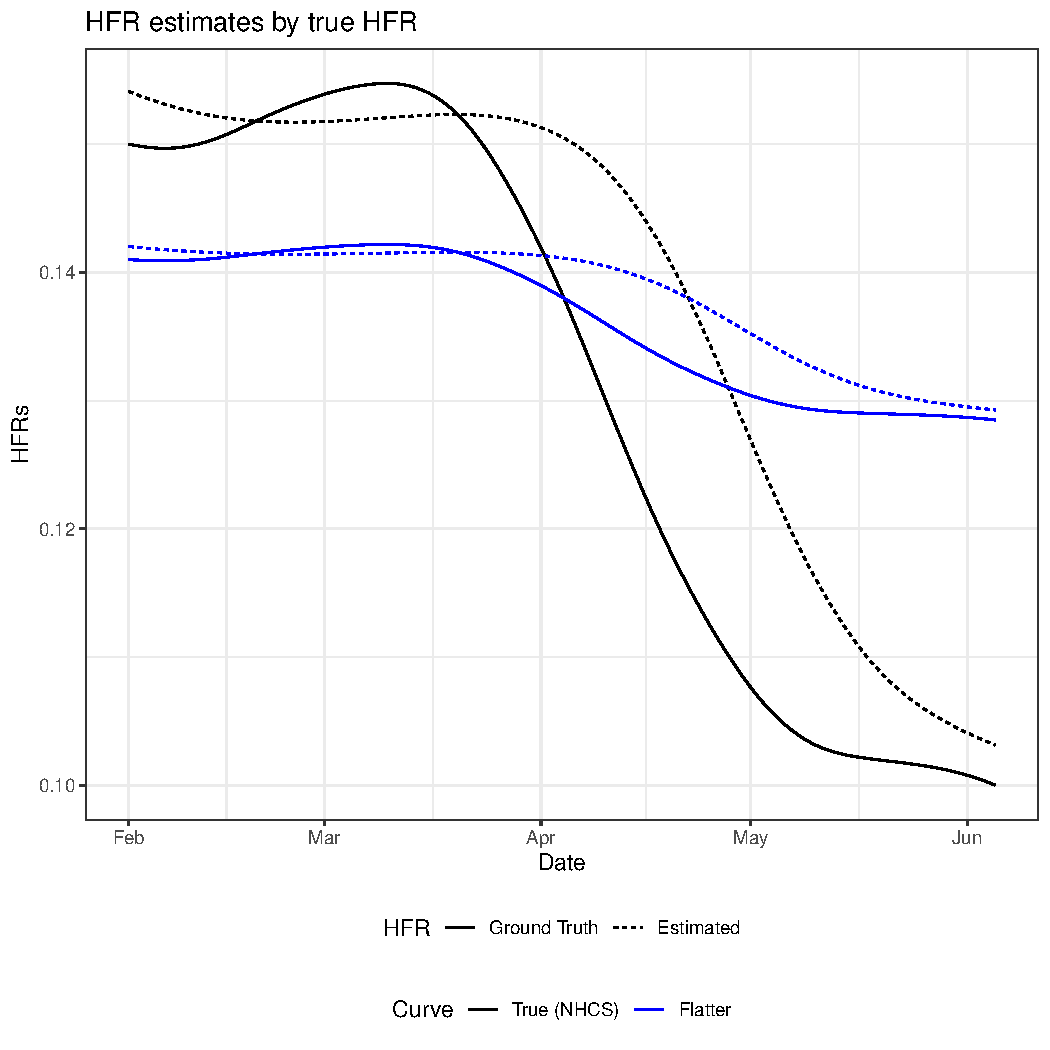
\includegraphics[width=\linewidth]{Figs/Simulated/toy_chging_hfr.pdf}
         \caption{}
         \label{fig:toy_hfr}
     \end{subfigure}
     % \hfill
     \begin{subfigure}[b]{0.32\linewidth}
         \centering
         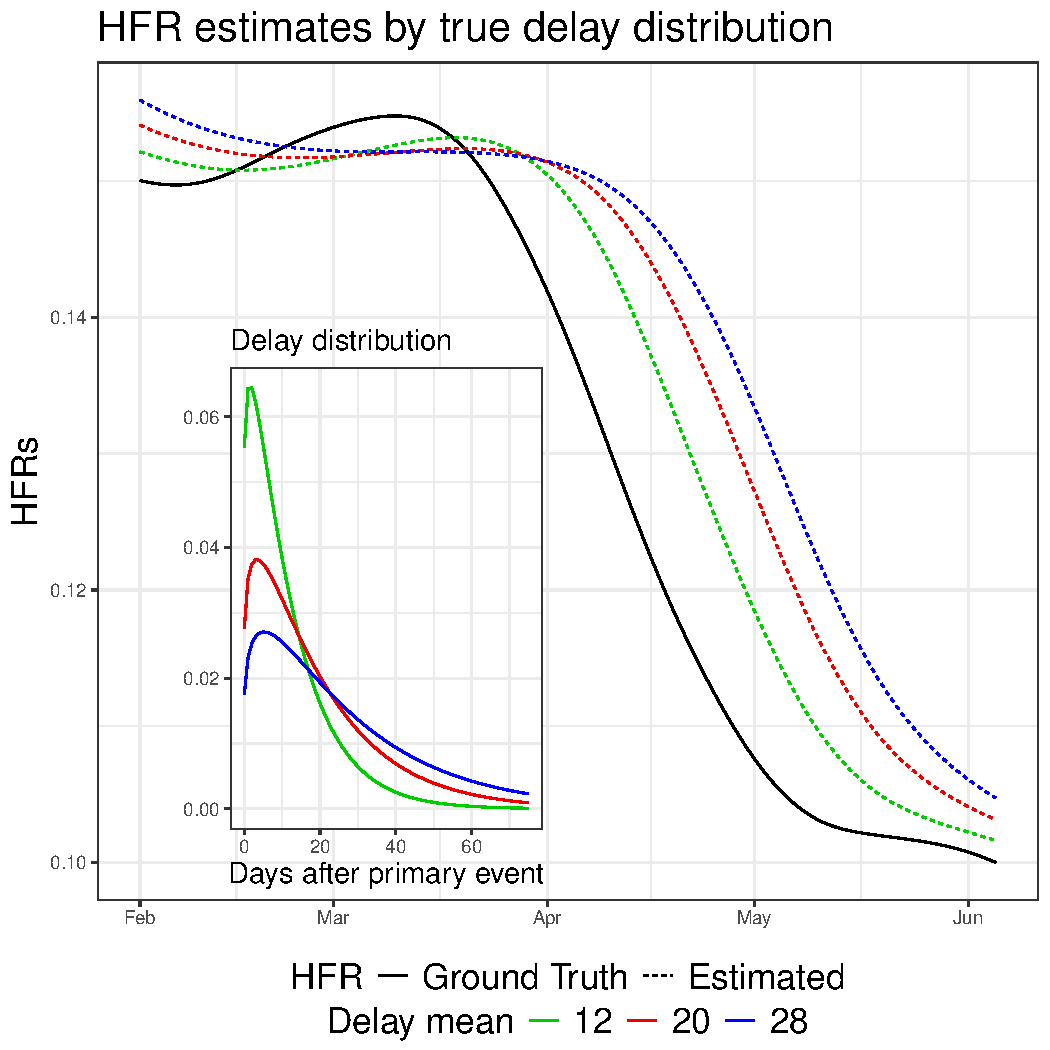
\includegraphics[width=\linewidth]{Figs/Simulated/toy_delay_distr.pdf}
         \caption{}
         \label{fig:toy_delay}
     \end{subfigure}
     % \hfill
     \begin{subfigure}[b]{0.32\linewidth}
         \centering
         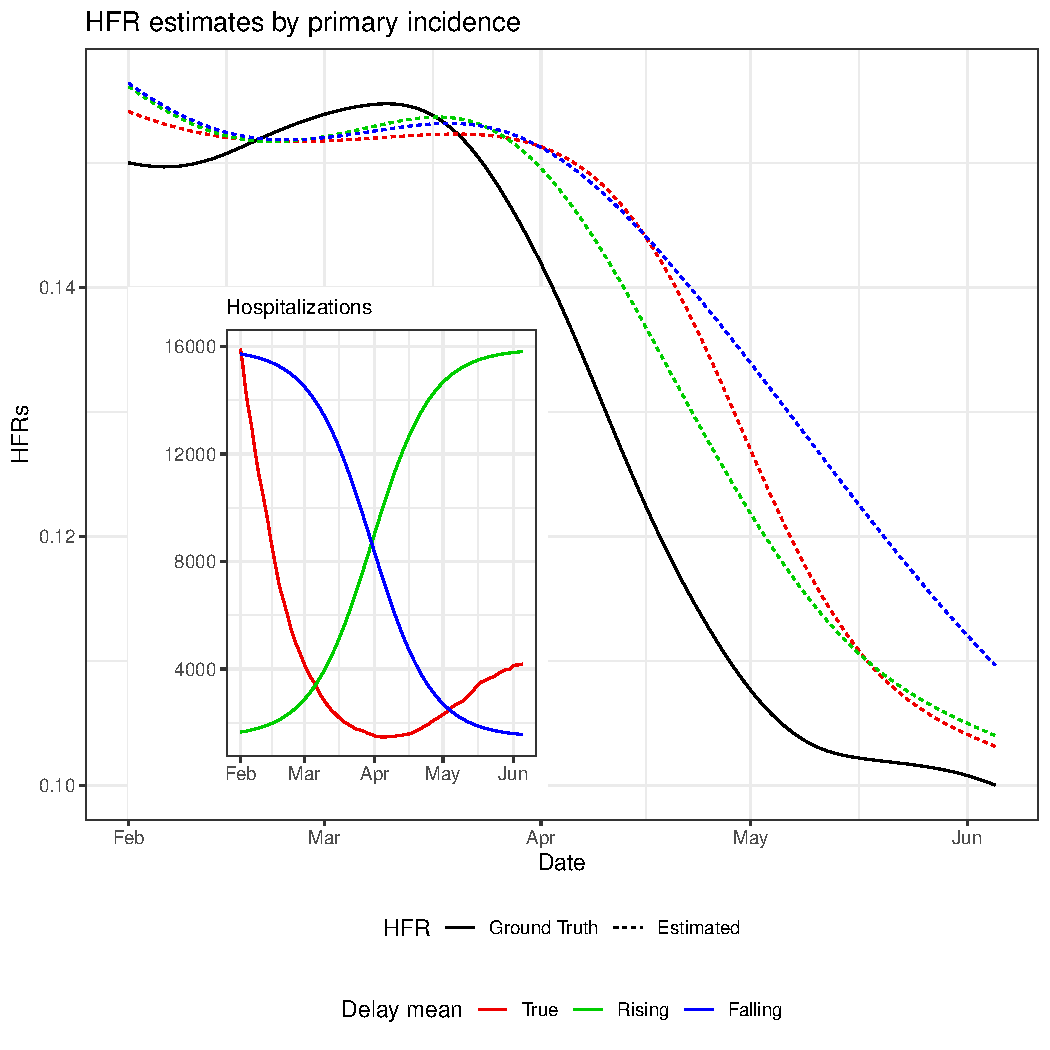
\includegraphics[width=\linewidth]{Figs/Simulated/toy_chging_primary.pdf}
         \caption{}
         \label{fig:toy_primary}
     \end{subfigure}
        \caption{Simple examples of severity rate bias to illustrate the three
        factors. Deaths were computed noiselessly from \eqref{eq:model}.
        Section~\ref{sec:setup} details data sources: 
        NHCS HFRs and HHS hospitalizations in early 2022,
        and delay distribution estimated with JHU deaths.}
        % , with
        % NHCS HFRs and HHS hospitalizations during early 2022. 
        % Panels \ref{fig:toy_hfr} and \ref{fig:toy_primary} 
        % use the delay distribution
        % estimated with JHU deaths (Section~\ref{sec:setup}).}
        \label{fig:bias_ex_main}
\end{figure}
% \end{adjustwidth}



% As noted previously, the convolutional ratio is equivalent to the lagged ratio if $\gamma$ is a point mass distribution at $\ell$. In this oracle setting, all secondary events occur after exactly $\ell$ days, a highly unrealistic situation. Nevertheless, if this is the case, then 
% $$
% \bias\left(\hat{p}_t^\ell\right) = \bias\left(\hat{p}_t^\gamma\right) = p_{t-\ell}-p_t.
% $$
% This toy setting and others are discussed in Appendix~\ref{apx:analysis}.
Appendix~\ref{apx:analysis} discusses toy settings in which the well-specified bias simplifies in elucidating ways.

\subsection{Misspecified analysis}\label{sec:misp}

The above section considered the bias of the convolutional ratio where the true delay distribution $\pi$ is known. We now consider the more general case, in which it is instead replaced with a plug-in estimate $\gamma$. Note the bias of the lagged estimator is a special case, where the plug-in distribution is a point mass at lag time $\ell$. 

\begin{proposition}\label{thm:MispBias}
Assume that the true delay distribution $\pi$ is constant over time and that its maximal length $d$ exceeds that of the plug-in distribution $\gamma$. 
Define $A_t^\gamma = \sum_{j=0}^d X_{t-j}\pi_j\, \big/\, \sum_{j=0}^d X_{t-j}\gamma_j$, which compares how the delay distributions convolve against the most recent primary incidence levels. The misspecified bias is
% The bias of this misspecified estimator can be expressed additively in terms of the rescaled oracle bias plus a misspecification error term.

\begin{equation*}
          \bias\left(\hat{p}_t^\gamma\right) = A_t^\gamma\bias\left(\hat{p}_t^\pi\right) + p_t\big( A_t^\gamma-1\big).
\end{equation*}
\end{proposition}

For the lagged estimator, \eqref{thm:MispBias} becomes
\begin{equation}\label{eq:LagBias}
         \bias\left(\hat{p}_t^\ell\right) = \frac{\sum_{j=0}^d X_{t-j}\pi_j}{X_{t-\ell}}\bias\left(\hat{p}_t^\pi\right) + p_t\left( \frac{\sum_{k=0}^d X_{t-k}\pi_k}{X_{t-\ell}}-1\right).
\end{equation}

Proposition \ref{thm:MispBias}, proven in Appendix~\ref{apx:proofs}, provides an
additive decomposition of the misspecified ratio's bias. In both terms,
$A_t^\gamma$ dictates the extent to which the misspecified distribution alters
the bias. The first term scales the oracle bias, whereas the other solely
expresses misspecification. Which of these two terms will dominate depends on
the true severity rate $p_t$, the oracle bias, and the ratio $A_t^\gamma$. If
oracle bias is small, for example, then its multiplicative scaling should have
relatively little effect, in which case the misspecification term may drive
bias. This seems to generally be the case in the simulated experiments in
Section~\ref{sec:results_sim}.

% \djmcomment{I think that Figure 2 needs a direct discussion somewhere in these
% next few paragraphs. Like ``Figure 2 illustrates\ldots''.} 
% \jmgcomment{Good idea. I've restructured this section accordingly. Along the way, I added some commentary about the misspecified convolutional ratio when primary incidence begins falling.}



% Suppose primary events have stabilized after falling for a long time (see April 2022 in Fig.~\ref{fig:misspecified}). If the plug-in delay distribution is
% too light-tailed, then $A_t^\gamma>1$, since it does not upweight distant dates
% with high primary counts. Therefore, this distribution inflates the oracle bias
% multiplicatively and adds positive misspecification bias. If primary events have
% consistently risen instead, then $A_t^\gamma < 1$, so the oracle bias term would
% shrink and the misspecification bias would be negative. This explains the
% negative bias of the light-tailed distribution in mid-January.  These relations
% may be more complicated if primary incidence has changed direction throughout
% the delay distribution.

How $A_t^\gamma$ affects bias depends on how the delay distributions convolve against the primary incidence curve. 
% The plug-in distribution $\gamma$ operates through its denominator, ${\sum_{j=0}^d X_{t-j}\gamma_j}$. 
When $\gamma$ is the oracle delay distribution $\pi$, $A_t^\gamma=1$. While this is not necessarily optimal, misspecification often exacerbates the bias.For example, suppose $\gamma$ has a similar shape as $\pi$, but a lower mean and lighter tail.
If primary events are rising sharply, $\gamma$ will place more weight on recent dates with high counts, and less on the low-count past. Put formally, $\sum_{j=0}^d X_{t-j}\gamma_j > \sum_{j=0}^d X_{t-j}\pi_j$, so $A_t^\gamma < 1$. 

$A_t^\gamma$ stays below 1 as primary incidence peaks and begins to decline, since $\gamma$ continues to upweight the current surge. 
Then, as incidence levels out, conditions flip. 
Because $\pi$ is more right-skewed than $\gamma$, it places more mass on the higher-count dates during the surge.
% $\gamma$ emphasizes the recent low counts, whereas $\pi$ places more mass on the high-count dates atop the surge. 
Correspondingly, $A_t^\gamma$ rises above 1. The opposite trends holds if $\gamma$ is heavier-tailed than $\pi$, with higher mean: $A_t^\gamma$ rises above 1 alongside primary incidence, stays high into the decline, and falls below 1 as incidence levels out. 
% Under rising cases $A_t^\gamma > 1$, and  $A_t^\gamma < 1$ after a fall. 

The lagged ratio has a point-mass delay distribution, $\gamma_k=\mathds{1}\{k=\ell\}$. This behaves  differently than the smooth distributions discussed above. When incidence rises, $X_{t-\ell}$ is considerably lower than $X_{t-\ell}$, so $A_t^\gamma>1$. As it later begins to fall, $A_t^\gamma$ switches below 1, since its denominator $X_{t-\ell}={\sum_{j=0}^d X_{t-j}\gamma_j}$ goes over the peak. Finally, $A_t^\gamma > 1$ as incidence flattens, since $\gamma_k$ has no tail with which to capture the higher-count dates. 

% The lagged estimator also exhibits interesting behavior as primary incidence falls from its peak. 
% Counts neared the peak $\ell$ days ago, so $X_{t-\ell}$ is approximately the maximum value of ${\sum_{j=0}^d X_{t-j}\gamma_j}$. 
% In contrast, a smoother distribution like $\pi$ will produce a smaller convolution due to its inclusion of lower counts before and after the peak. 
% As a result, $A_t^\ell<1$, contributing negative bias.

% In this case, the lagged ratio roughly obtains the worst-case delay distribution in Proposition~\ref{thm:MispBias}. 
More generally, $A_t^\gamma$ is most extreme when $\gamma$ is a point-mass distribution at the maximal or minimal values of $X_{t-d}, \ldots, X_t$. This inevitably occurs with the lagged estimator as its convolution sweeps across the primary incidence curve. In contrast, the convolutional ratios do not reach such extremes by nature of their smooth delay distributions. 
Hence, the lagged ratio is likely to have larger fluctuations of $A_t^\ell$, and thus higher bias.
In some settings, it may even attain the worst-case delay distribution in Proposition~\ref{thm:MispBias}. 

Figure~\ref{fig:misspecified} illustrates these biases. As anticipated, $A_t^\gamma$ with a lighter-tailed gamma distribution is less than 1 while hospitalizations surge in January 2022. It then spikes when they bottom out in March and April. The heavy-tailed distribution follows the opposite pattern, switching from high to low around March 1st. For the lagged ratio, $A_t^\ell$ spikes high to low to high again. Moreover, its peaks are higher than its smooth counterparts.

These patterns translate accordingly into the biases themselves. The lagged ratio has higher bias than the convolutional ratios across its three spikes. In general, curves with $A_t^\gamma>1$ have more positive bias than the oracle ratio, while $A_t^\gamma<1$ corresponds to negative bias. This aligns with the misspecification term in Proposition~\ref{thm:MispBias}. Analysis in Section~\ref{sec:results_sim} further indicates that $A_t^\gamma$ predominantly affects bias through this term. 

% In some cases,  $\gamma_k=\mathds{1}\{k=\ell\}$ can be thought as a light-tailed
% distribution. It assigns all its mass at $\ell$ --- chosen to be around the mean
% of $\pi$ --- and none in the long tail of $\pi$. 
% In the flattened-out period
% around April 2022, the lagged estimator has similar positive bias as the
% short-tailed convolutional ratio. 

% Overall, however, the lagged estimator's bias is more subtle because it relies
% exclusively on primary incidence $\ell$ days ago. When counts rise sharply
% between $t-\ell$ and $t$, then $A_t^\ell>1$ due to its small
% denominator. This contrasts with the smooth, light-tailed $\gamma$ described
% above, which emphasizes recent high counts. 
% Figure~\ref{fig:misspecified}
% highlights this divergence in behavior as hospitalizations peak in mid-January. 

% The lagged estimator also has interesting behavior as primary incidence falls from its peak. The denominator of $A_t^\ell$ is large, since counts neared the peak $\ell$ days ago. Meanwhile, the numerator is smaller due to its inclusion of lower counts before and after the peak. As a result, $A_t^\ell<1$, contributing negative bias. Misspecified smooth delay distributions will be less biased under these conditions, since they incorporate the lower counts into the denominator of $A_t^\gamma$. 
% This accounts for the lagged ratio's spurious dip in February 2022. 

% Note the denominator of $A_t^\gamma$, ${\sum_{j=0}^d X_{t-j}\gamma_j}$, is most extreme when $\gamma$ is a point-mass distribution at the maximal or minimal values of $X_{t-d}, \ldots, X_t$. This inevitably occurs with the lagged estimator as its convolution sweeps across the primary incidence curve. In contrast, the convolutional ratios do not reach such extremes by nature of their smooth delay distributions. 
% This explains why in Figure~\ref{fig:misspecified}, the ratio $A_t^\ell$ fluctuates furthest away from 1 for the lagged estimator. 
% Hence, the lagged ratio can occasionally be understood as providing the worst-case delay distribution in Proposition~\ref{thm:MispBias}.

\begin{figure}
    \centering
    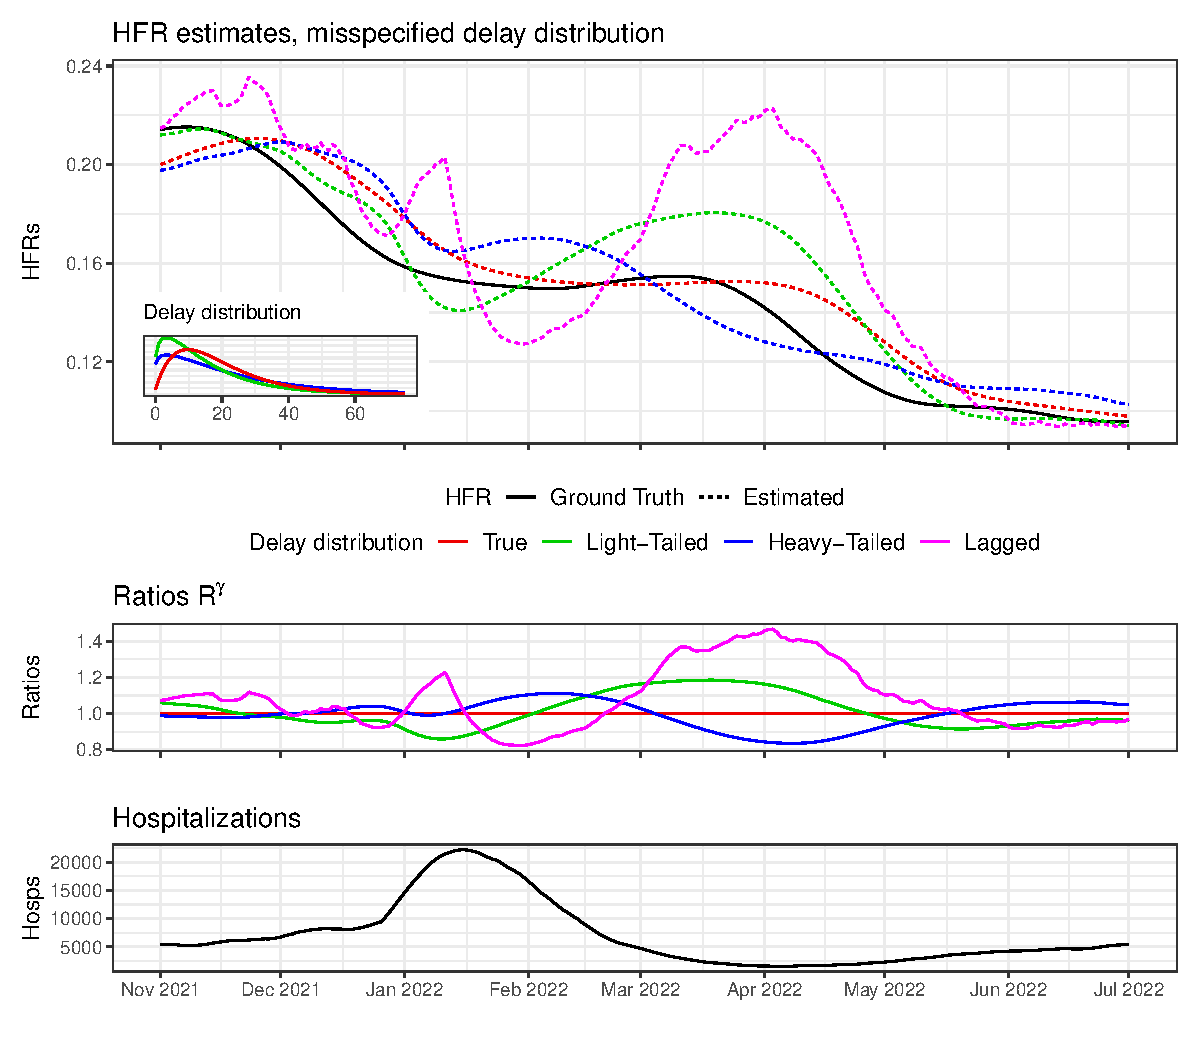
\includegraphics[width=.8\linewidth]{Figs/Simulated/toy_misp.pdf}
    \caption{HFR estimates under misspecification. HHS hospitalizations, NHCS HFRs, and noiseless deaths from \eqref{eq:model} (Section~\ref{sec:setup}). True delay distribution is gamma with mean of 20 days. 
    Convolutional ratio estimates use oracle delay distribution, misshapen gammas (mean 16 and 24), and point mass at correlation-maximizing lag (16).}%(i.e. lag) at oracle mean
    \label{fig:misspecified}
\end{figure}

% \textcolor{brown}{For...}


\subsection{Experimental setup}\label{sec:setup}
% \djmcomment{I wonder if it wouldn't be better to put this section (2.1) as the last section before you move to Results rather than the first?}
% \jmgcomment{Tricky. I had originally had it there, but Addison argued the opposite: The analysis has 2 figures that use this data, so it makes sense to introduce earlier. I could go either way.}
\jmgcomment{Should it be its own whole section?}
% \djmcomment{References. I personally try to use the \texttt{cleveref} package so
% that I can write something like ``In \textbackslash cref$\{$sec:blah$\}$\ldots''
% which gets typeset as ``In Section 3\ldots''. You can use \textbackslash
% autoref$\{$sec:blah$\}$ (part of \texttt{hyperref} that you're already using) to get
% similar results, though it is a bit more fragile. Feel free to do neither.
% However, 2 things that I think are important: (1) you should do
% Section$\sim$\textbackslash ref\{sec:blah\} with the tilde to make sure that
% references don't get split across lines; (2) equations should be written as
% either Equation$\sim$\textbackslash eqref$\{$eq:3$\}$ or Eq.$\sim$\textbackslash
% eqref\{eq:3\} rather than just \textbackslash eqref\{eq:3\}. Some journals
% require one or the other, and I don't really have a preference, as long as it's
% consistent.}

\paragraph{Hospitalization-fatality rate.}
Our experiments analyze the HFR throughout COVID-19. 
While HFR is less commonly reported than CFR, it has a few advantages as an object of study.
Firstly, time-varying HFR estimates for the US can be validated with a line list. The ``Validation data" section below describes this in detail. To our knowledge, no such resource exists for CFR. 

In addition, hospitalization reporting was much more complete than case reporting throughout the pandemic. Hospitals were mandated to report new daily admissions to the Department of Health and Human Services (HHS) or face penalties \citep{HHS2023}. 

Lastly, our analysis assumes the true time-to-death delay distribution has non-negative support. This holds true for HFR, since COVID hospitalizations are aligned by admission date. 
% Lastly, the delay distribution for HFR is indeed supported on integers starting at $k=0$, since hospitalizations are aligned by admission date. 
For CFR, however, cases may be reported after deaths due to long reporting delays. 
Cases were sometimes reported up to 45 days after infection \citep{Jahja2022}; meanwhile, \citet{Lancet_delays} studied a cohort in which the median infection-to-death time was only 18 days.
Nevertheless, negative case-to-death delays are uncommon enough that the same findings should apply for both CFR and HFR \citet{nishiuraEx2, UKdelay}.

\paragraph{Aggregate data.}
To estimate real-time HFRs, we use daily hospitalizations and deaths as
available in
the \texttt{epidatr} API, developed by the Delphi Group. Like HHS for
hospitalizations \citep{HHS2023}, John Hopkins University (JHU) provided the
definitive resource for real-time death counts \citep{JHUepidatr}. These counts
reflect the times at which deaths were reported to health authorities, not
necessarily when they actually happened. Therefore raw JHU death counts are
highly volatile due to reporting idiosyncrasies like day-of-week effects and
data dumps. As a result, we used a 7-day trailing average of counts. 

Because the daily aggregates from JHU and HHS were updated over the course of
the pandemic, we use both the counts available in real time as well as their
finalized versions. Occasionally, the most recent date with available counts
lagged several days behind the present. To account for this, we estimated HFRs
each week, using real-time data that was available two days after each date. 
Therefore the real-time estimates are actually a two-day backcast of the HFR.
In the rare event that requested counts were still unavailable, we imputed the
value with the most recently observed data. 
%Finally, we smoothed counts over the previous 7 days. 

\paragraph{Hyperparameters.}
The ratio estimators studied require choices of lag and delay distribution. 
% The two ratio estimators \eqref{eq:lagged} and \eqref{eq:conv} require choices
% of lag and delay distribution. 
% \djmcomment{I try to avoid referring to future
% equations. So this is another reason to consider moving this subsection to the
% end. In fact, I might put this paragraph right at the beginning of Section 3
% (before 3.1). It's a good summary of what comes next there.} 
Appendix~\ref{apx:robustness} evaluates the
robustness of findings against different hyperparameter values. The experiments
in Section~\ref{sec:results_real} use a lag of 20 days, which maximizes the
cross-correlation between hospitalizations and deaths over all time
\citep{atlantic}. 

We let the delay distribution be a discrete gamma, a common
choice \citet{delay_distrs}. We set its mean to this oracle lag, as lags are often chosen to be the
mean of the delay distribution. This mean of 20 matches nicely with a UK study
that finds a median hospitalization-to-death time of 11 days \citep{UKdelay},
and a CDC report that 63\% of COVID deaths are reported within 10 days
\citep{cdc_deaths_demographic_geographic_2023}. 
We set the standard deviation to 18, because the delay distributions fit by the UK study had standard deviations that were roughly 90\% of their means. 

It is worth noting that conditions in the UK may be quite different from the US. However, we use this paper's findings because it provided the most comprehensive information on COVID hospitalization-to-death delay distributions.

\paragraph{Validation data.}
While the true HFRs are unknown, there are sound ways to approximate them. One such approach is to use line-list HFRs from the National Hospital Care Survey \citep{NHCS2023}. The NHCS recorded weekly HFRs from inpatient deaths in a representative subset of 601 hospitals across the US.

HFRs from aggregate hospitalization and death counts are significantly higher than those from NHCS because not all deaths occur in hospitals. A CDC analysis reported the percentage of inpatient deaths every month from 2020 through 2022; roughly 60\% of COVID deaths occurred in hospitals in 2022, down from nearly 70\% in 2021 and 2022. To account for non-inpatient deaths, we divided the NHCS curve by these percentages. Finally, we smoothed the resulting HFRs with a spline. To do so, we used the \texttt{smooth.spline} function in \texttt{R}, which chooses the smoothness hyperparameter with generalized cross validation. 

The NHCS curve is a useful benchmark to judge the fidelity of our HFR estimates. Of course, its values may be inaccurate because it surveys a relatively small subset of hospitals. Results in Section~\ref{sec:results} suggest it is too high in late 2022. Appendix~\ref{apx:alt_gt} discusses other approximations of ground truth HFRs. 
% We considered two other sources for ground truth HFRs, discussed in Appendix~\ref{apx:alt_gt}. Unlike NHCS, these HFRs are obtained from aggregate counts, not line-list data. Fortunately, they are fairly consistent with the rescaled NHCS data. Of course, the NHCS curve is merely an approximation for the ground truth; its values, especially after mid-2022, may be incorrect. Nevertheless, it is a useful benchmark to judge the fidelity of our HFR estimates.

\section{Results}\label{sec:results}

In this section, we explore the performance of the ratio estimators in greater depth. 
We analyze HFR estimates on real data in Section~\ref{sec:results_real}, and simulated data in Section~\ref{sec:results_sim}. Throughout both, we continue to use aggregate hospitalization counts from HHS throughout the COVID-19 pandemic. 

\subsection{COVID-19 data}\label{sec:results_real}

\begin{figure}
     \centering
     \begin{subfigure}[b]{0.55\linewidth}
         \centering
         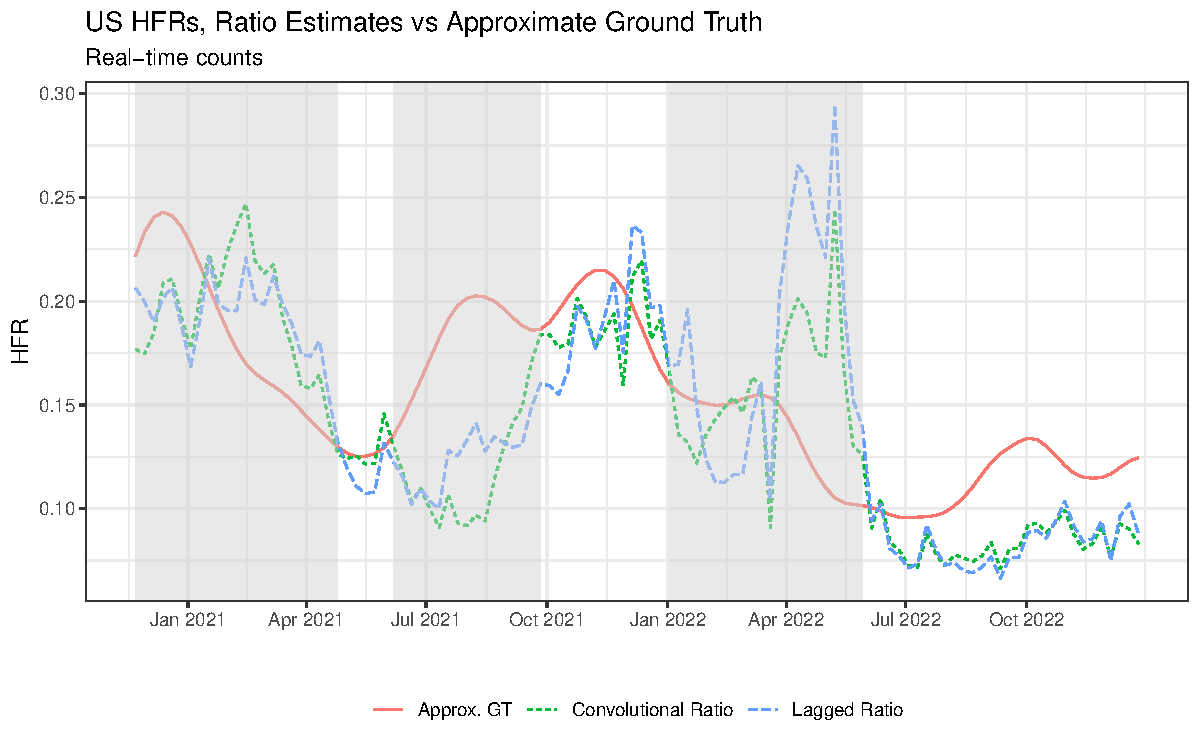
\includegraphics[width=\linewidth]{Figs/Real/US_ests_realtime.pdf}
         \caption{Comparing convolutional and lagged ratios against approximate ground truth.}
         \label{fig:basic_est_vs_gt}
     \end{subfigure}
     \hfill
     \begin{subfigure}[b]{0.4\linewidth}
         \centering
         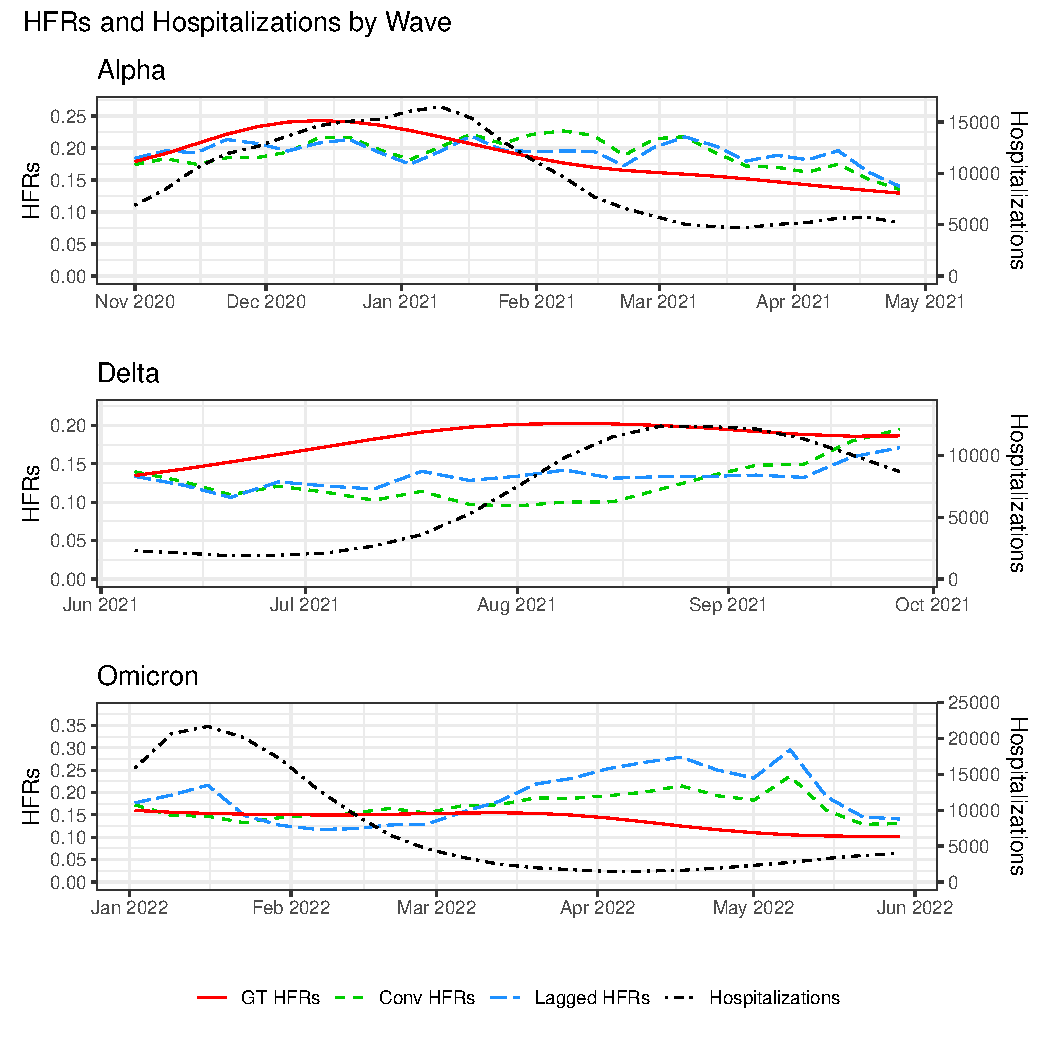
\includegraphics[width=\linewidth]{Figs/Real/hfrs_by_wave.pdf}
         \caption{HFRs and hospitalizations in three periods with major bias.} 
         \label{fig:wave}
     \end{subfigure}
        \caption{Convolutional ratio estimates are biased regardless of which delay distribution is selected. Real-time counts, Nov. 2020 - Dec. 2022. Biased periods of major waves are highlighted.}
        \label{fig:basic_est_vs_gt_figs}
\end{figure}

% Figure \ref{fig:basic_est_vs_gt_figs} highlights the bias of these ratio
% estimators 
% \djmcomment{as described in Propositions 1 and 2 when applied to\ldots}. 
Figure \ref{fig:basic_est_vs_gt_figs} highlights the poor performance of the ratio estimators on the data described in Section~\ref{sec:setup}. 
As described in Propositions \ref{thm:OracleBias} and \ref{thm:MispBias}, the bias is consistent and nontrivial, especially for the lagged estimator.
Both the lagged and convolutional ratios respond very slowly to
changes in the HFR. As the HFR declines following the wave in winter 2021, both
ratios remain near 0.2 for several months. More troublingly, they are very slow
to detect the rising HFR in the early Delta period (summer 2021). %A central
If the purpose of these estimators is to inform stakeholders of increased risks
in real time, they fail during the Delta surge.

The most significant bias comes in the middle of the Omicron wave in spring 2022. 
In this period, the HFR remains around 15\% until April, then sharply declines to 9\% two months later. The lagged ratios first fluctuate above and below the true HFRs. Subsequently, both estimates surge as the true HFR nears its nadir, with the lagged ratio nearing 30\%. This dramatic upswing signals a serious false alarm. 
The analysis in Sections~\ref{sec:ws_analysis} and \ref{sec:misp} explain each
of these failure cases. We start by analyzing the convolutional ratio with
respect to the well-specified bias expression in Proposition \ref{thm:OracleBias}.
While this expression assumes that the true delay distribution is known, we found
that different choices of delay distribution generally yield the same bias
(Appendix~\ref{apx:robustness}). This indicates that our estimates may not be far
from the oracle ratio.

First, Proposition \ref{thm:OracleBias} indicates that the bias moves in the opposite direction of the true severity rate. This occurs during the Delta wave, when the HFRs rise well before the ratio estimates do. Conversely, falling HFRs produce positive bias, as observed in the original and Omicron waves.
% Falling HFRs correspond to positive bias, as observed in early 2021 and 2022. 
Second, the enormity of the bias during Omicron can partially be attributed to the precipitous decline in hospitalizations, as falling primary incidence has been shown to exacerbate the bias. Average daily hospitalizations declined from over 20,000 in mid-January to only 1,500 by April 1. 
Finally, the delay distribution is relatively long with JHU deaths due to its alignment by report date. This is shown to have a substantial impact on the bias, as analyzed in Appendix~\ref{apx:NCHS_deaths}.
Third, the misspecification analysis explains central discrepancies between the
convolutional and lagged ratios. The lagged ratio's erratic behavior during
Omicron is almost identical to the simulated results in
Figure~\ref{fig:misspecified}. This bias is likely due to changes in
hospitalization counts, which affect $A_t^\ell$ in Proposition \ref{thm:MispBias}.
Finally, the lagged ratio is briefly less negatively biased in August 2021, during the Delta wave. Like the spike in January 2022, this can be explained by the sharp rise in hospitalizations. The surge causes $A_t^\ell$ to rise above 1, so the additive term in \ref{thm:MispBias} is positive. This briefly offsets the negative oracle bias, bringing the lagged ratio closer to the true HFR. Similarly, the lagged bias is less \textit{positive} in February 2021. Here, $A_t^\ell < 1$ due to falling hospitalizations, so the additive term is negative. 
% Our analysis attributed the bias to $A_t^\ell$ in Proposition \ref{thm:MispBias}, affected by changes in hospitalization counts.

We performed several robustness checks to assess the stability of these findings. Appendix~\ref{apx:robustness} explores the effect of different hyperparameters and locations. By and large, the ratio estimators yield roughly the same bias regardless of these considerations. It also compares HFR estimates using finalized counts, rather than the data available in real time. This exploration finds that the observed biases could not be attributed to real-time reporting issues. 

\subsection{Simulated data}\label{sec:results_sim}

We further evaluated these methods in a variety of simulation settings. Given a series of time-varying HFRs $p_t$ and delay distribution $\pi$, deaths are defined without noise from \eqref{eq:model}:
$$Y_t = \sum_{k=0}^d X_{t-k} \mathbb{P}(\text{die at $t$}\given\text{hosp at }t-k) = \sum_{k=0}^d X_{t-k} \pi_k p_{t-k}.$$

Like the experiments in Sections~\ref{sec:ws_analysis} and~\ref{sec:misp}, we
used finalized HHS hospitalization counts. However, the simulations in this
section evaluate performance over a two-year period, with a broader range of
underlying HFR curves. To supplement the NHCS HFRs, we mimicked the opposite
trend by inverting and rescaling them. We also modeled a stationary HFR of 10\%
over all time. As in Section~\ref{sec:setup}, the delay distributions were again
gamma with standard deviation 0.9 of their mean. We experimented with means of
12 and 24 to illustrate a short and long delay distribution. 

To elucidate the oracle bias in Proposition \ref{thm:OracleBias}, we let the convolutional ratio use the true delay distribution. For the lagged ratio, $\ell$ was again chosen to maximize the cross-correlation between hospitalizations and deaths. We also experimented with the mean of the delay distribution, as advocated by \citet{lagged_chinese}. Figure \ref{fig:sims_mean_lag} in Appendix~\ref{apx:misc} shows the results are similarly unstable.


\begin{figure}
    \centering
    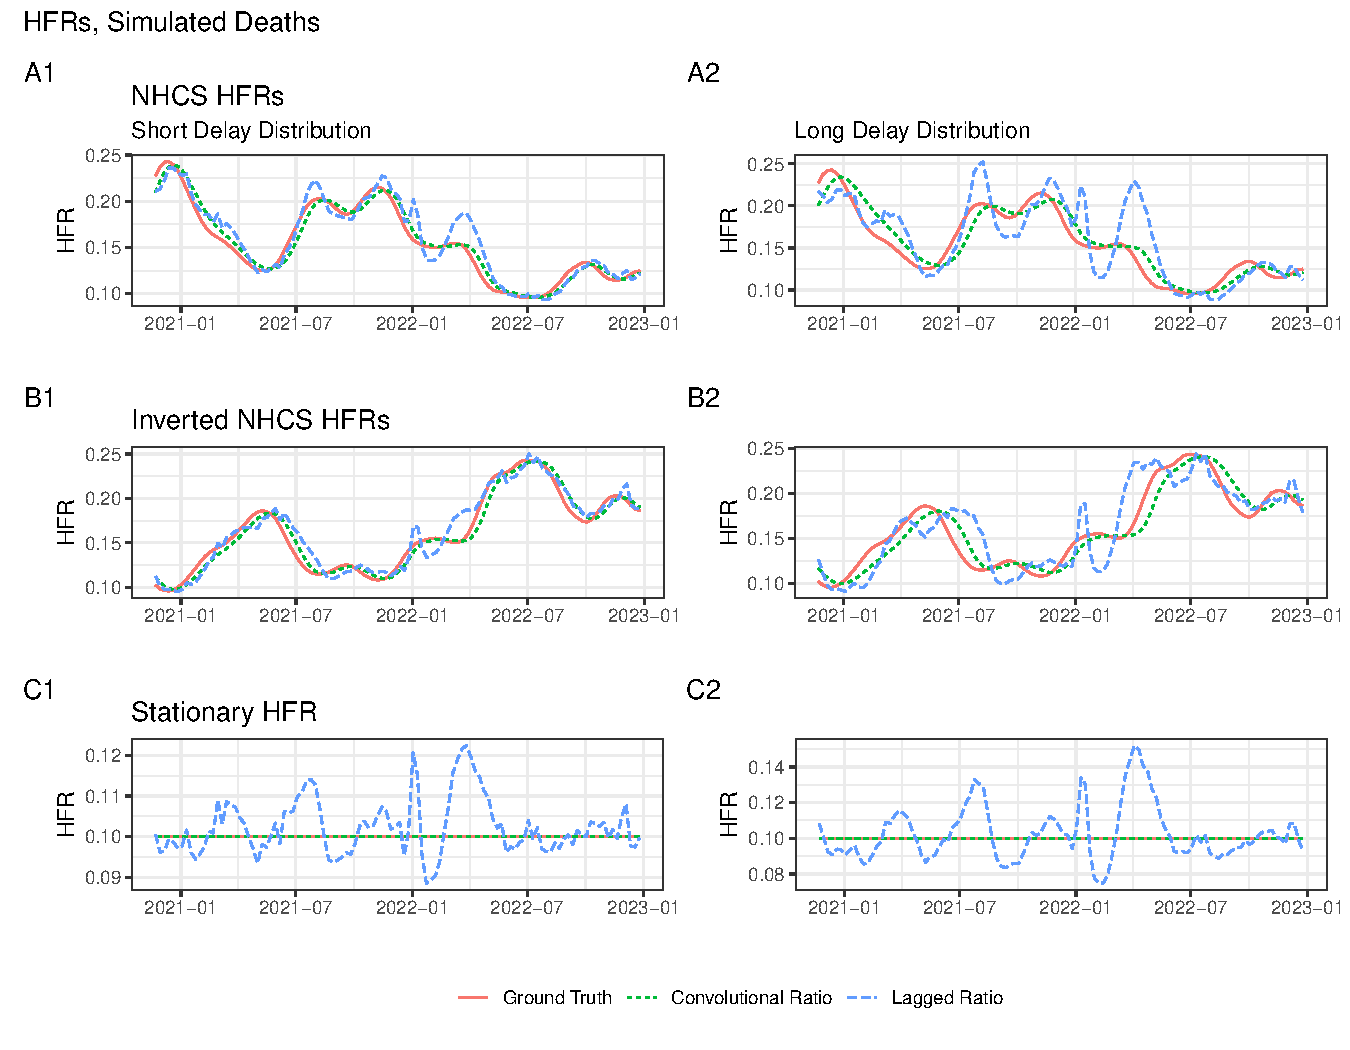
\includegraphics[width=\linewidth]{Figs/Simulated/simulated_results.pdf}
    \caption{True and Estimated HFRs from Simulated Deaths. First column has short delay distribution, second has long.}
    \label{fig:sims}
\end{figure}

Figure \ref{fig:sims} displays the results on the six settings of delay distribution and HFR. 
% Consequently, $\hat{p}_t^\gamma = p A_t^\gamma$. 
%so the $A_t^\gamma$ curve merely rescales the estimated HFRs by a factor of $p$. 
Matching expectations, HFRs are significantly more biased given the longer underlying delay distribution. 
In all three HFR settings, the lagged ratios swing more widely. For example, when the true HFR is a constant 10\%, they peak at 12\% under the light-tailed distribution, compared to 15\% with the heavy tail. The oracle convolutional ratio does not share the lagged estimator's dramatic oscillations. Rather, it tracks the general shape of true curve, albeit at a delay. For the NHCS HFRs, the average delay was 5 days for the light-tailed distribution, and 12 days with heavy tail; these delays were 6 and 15 days for the inverted curve. (To compute the average delay, we again took the maximal cross-correlation between the two series.)

% In general, the oracle convolutional ratio performs much better than the lagged estimator. Our analysis accounts for this wide gap in performance. In the case of a stationary severity rate, for example, Proposition \ref{thm:OracleBias} assures the oracle convolutional ratio is unbiased. But if the delay distribution is misspecified, Proposition \ref{thm:MispBias} expresses the resulting bias via the ratio $A_t^\gamma$. This quantity does not depend on the severity rate, so the bias moves in similar trajectories across the three HFR settings. 
In general, the oracle convolutional ratio is much more accurate than the lagged estimator. The analysis in Section~\ref{sec:misp} accounts for this wide gap in performance. The lagged bias moves in ways that align with our observations.

Proposition \ref{thm:MispBias} expresses the lagged bias via the rescaled oracle bias plus a misspecification term, both of which depend on the ratio $A_t^\gamma$. 

These ratios $A_t^\gamma$ are visualized in Figure \ref{fig:sims} as rescaled HFR estimates in the stationary case.
% In addition to the HFR curves, it also visualizes the ratios $A_t^\gamma$, which merely rescale the HFR estimates in the stationary case. 
Given a constant rate $p$, the oracle convolutional ratio is unbiased, so Proposition \ref{thm:MispBias} reduces to $\mathbb{E}[\hat{p}_t^\gamma] = p A_t^\gamma$. Furthermore, $\mathbb{E}[\hat{p}_t^\gamma] = \hat{p}_t^\gamma$, as our setup simulates deaths without noise. Consequently, $A_t^\gamma = \frac{\hat{p}_t^\gamma }{p}$. 

The analysis in Section~\ref{sec:misp} explains these trajectories. During the Delta and Omicron waves, rapid rises in hospitalizations produced high values of $A_t^\ell$. This accounts for the spikes in August 2021 and January 2022, across all 3 HFR settings. Positive bias is also expected when hospitalizations have leveled out from a decline. This consistently occurs in spring 2022, with $A_t^\ell$ reaching 1.2 and 1.5 for the short and long distributions. Lastly, the lagged estimator should have negative bias as primary events fall. We observe this in Delta (September 2021) and Omicron (Februrary 2022). 

% Not sure if these two paragraphs belong in the discussion. They're analytical, but don't belong in Section 2.4 because they rely on these empirical results. 
The misspecified bias (Proposition \ref{thm:MispBias}) rescales the oracle bias and adds a misspecification term. Studying Figure \ref{fig:sims}, we observe the misspecification term tends to dominate when $A_t^\gamma$ strays away from 1. To understand this, consider periods in which the oracle bias is negative. Here, the oracle and misspecification terms are at odds with each other. 
When $A_t^\gamma > 1$, it both amplifies the negative oracle bias and adds positive misspecification bias. The opposite effect occurs when $A_t^\gamma<1$. 
% $A_t^\gamma > 1$ amplifies the negative bias while adding positive misspecification bias, whereas $A_t^\gamma<1$ has the opposite effect.

Invariably, the lagged ratio's bias moves in the direction of the misspecification term $p_t(A_t^\gamma-1)$. Under the true NHCS HFRs, for example, the lagged estimates spike with $A_t^\ell$ in August 2021. In the inverted setting, the lagged bias tracks the down-up-down motion of $A_t^\ell$ during the first five months of 2021. That the misspecification term wins out in these conflicting settings indicates it accounts for a disproportionate amount of the bias. 

For a further example, consider the bias at April 2022 in panel A2. The true HFR is 14\%, with the convolutional ratio nearby at 15\%. Meanwhile, the lagged ratio peaks at 22.5\%, driven upwards by an $A_t^\ell$ of $1.5$. Decomposing the lagged bias of $8.5\%$ with Proposition \ref{thm:MispBias}, the oracle term $A_t^\ell \text{Bias}(\hat{p}_t^\pi)$ equals only $1.5\%$; meanwhile, the misspecification term $p_t(A_t^\ell-1) = 7\%$, accounting for the majority of the bias. 

\section{Discussion}

Our analyses illustrate that practitioners should take caution when using
time-varying severity ratio estimators. They exhibit considerable bias when severity rates
change, particularly the popular lagged ratio estimator. A major purpose of these
estimators is to inform stakeholders of changing risks in real time; this bias
indicates they may fail to do so in a reliable manner.

% It may not be possible to infer about the oracle bias, since the true severity rates are unknown. However, understanding the central importance of the misspecification term in Proposition \ref{thm:MispBias} enables us to make broad heuristics about biases observed in practice. 
Analyzing the lagged ratio enables us to make real-time heuristics about its performance in practice. Proposition \ref{thm:MispBias} decomposes its bias into oracle and misspecification terms, the latter of which has been shown to dominate. Based solely on the primary incidence curve, we can expect the lagged ratio to make the following errors:
\begin{enumerate}
    \item Unreasonably high severity estimates when primary incidence is rising quickly;
    \item Rapid declines when primary incidence is falling quickly;
    \item Unexpected surges when primary incidence has leveled out after falling. 
\end{enumerate}

Practitioners can adjust their reactions accordingly when these bias patterns occur in real time. For example, if the lagged HFR spikes shortly after hospitalizations reach a stable low, a savvy epidemiologist can temper her alarm with the knowledge it may well be spurious.

While the lagged ratio is ubiquitous in practice, our analysis of its
drawbacks suggests other aggregate estimators should be favored. Figure
\ref{fig:sims} showed the oracle convolutional ratio is much more
accurate. 
% Even with a rough estimate of the delay distribution, 
% it generally displayed improved stability and performance (Figures \ref{fig:misspecified},
% \ref{fig:basic_est_vs_gt_figs}, and \ref{fig:sims}) --- though it still has large bias.
It still outperformed the lagged ratio given a misspecified delay distribution, though its bias was also large (Figures \ref{fig:misspecified} and \ref{fig:basic_est_vs_gt_figs}).
% While \eqref{eq:nish} from \citet{nishiura} is widely used to compute stationary or
% average HFRs, we have not come across any applications for the time-varying
% case.


% Given the drawbacks of these methods, alternative approaches may be preferable when there is reason to believe the true rate is changing. If possible, severity rates can be obtained from line-list data after accounting for right censoring. These rates can then be scaled to a broader population with careful demographic adjustment \citep{verity2020estimates}. 

% More commonly, only aggregate data is available, especially in real time. In that case, other methods may outperform these ratios. \citet{fusedlasso} propose estimating all severity rates at once with a Fused Lasso model, using the relation in \eqref{eq:model}. Unlike the other approaches, this method is inherently forward-looking, where rates at $t$ are exclusively used to produce secondary events after $t$. However, it may suffer from other sources of bias. It is inclined to estimate smoothly-changing severity rates as piecewise constant, and may yield unstable real-time estimates due to scarce data at the tail.

% \citet{fusedlasso} proposed a alternative approach which differs sharply from the ratios discussed in this paper. 
\citet{fusedlasso} proposed an approach that differs considerably from the ratios discussed in this paper. 
The method estimates all historical severity rates at once, using the relation in \eqref{eq:model} to fit a fused lasso model. This estimator is inherently forward-looking, where rates at $t$ are exclusively used to produce secondary events after $t$. Given regularization parameter $\lambda$, current time $T$, and start time $t_0$, the fused lasso estimates

$$\hat{p}^\text{FL} = \text{argmin}_{p \geq 0} \sum_{t=t_0}^T (Y_t-\sum_{j=0}^d X_{t-j}\gamma_j p_{t-j})^2 + \lambda\sum_{t=t_0-d+1}^{T}\lvert p_t - p_{t-1}\rvert.$$

This estimator is not succumb to the issues of the backward-looking ratios. However, it may suffer from other sources of bias. It is inclined to estimate smoothly-changing severity rates as piecewise constant, and may yield unstable real-time estimates due to scarce data at the tail. 
Thorough investigation of its performance is a promising object for future study.

Future work could generalize the above approach beyond piecewise constants. The fused lasso is a special case of trend filtering, a nonparametric regression technique that fits piecewise polynomials \citet{Tibshirani2014}. Higher-order curves may better model trends and improve performance. \citep{Jahja2022} applies trend filtering to a similar deconvolution problem, reconstructing latent infections from case reports. Its insights on tail regularization may be useful to stabilize severity estimates. 

\citet{UKpaper} also proposed a forward-looking method, this one a ratio between relevant primary and secondary events. However, this method is not applicable in real time, as it uses secondary events after $t$ to compute the severity rate. Nevertheless, it is a useful tool for retrospective estimation. 

Another retrospective tool is aggregate COVID deaths from NCHS, a resource that
was not available in real time (Appendix~\ref{apx:NCHS_deaths}). Unlike JHU,
whose aggregates align deaths by report date, NCHS counts deaths on the day the
actually occurred. As a result, the mean of its delay distribution is
considerably lower, so it produces more accurate ratio estimates (Figures
\ref{fig:sims} and \ref{fig:jhu_vs_nchs}). Analogously, bias is a more serious
issue with earlier primary events. For example, case- or infection-fatality
ratios may be more biased than hospitalization-fatality ratios. 

Severity rates may be biased in ways beyond the statistical bias our work
focuses on. 
In Section~\ref{sec:setup}, we mentioned that 
HFR estimation from aggregates is subject to survivorship bias --- 
the failure to account for deaths that occurred outside the hospital \citep{lipsitch2015potential}.
% Section~\ref{sec:setup} mentioned, for example, the fact that
% estimating HFR from aggregates fails to address the large proportion of deaths
% that occur outside the hospital; \citep{lipsitch2015potential} refers to this as
% ``survivorship bias." 
Under-reporting is another central challenge, particularly for CFR.
% Another central challenge, this one for CFR estimation, is under-reporting.
Not all infections are reported, reporting rates change across time, and severe
cases are more likely to be reported than mild cases.
\citet{reich2012estimating} proposed an estimator for a time-invariant
\textit{relative} CFR --- the ratio of CFRs between groups --- that learns these
latent reporting rates via the EM algorithm \citep{EM}. \citet{anastasios}
applied this in the context of COVID-19, analyzing how the chosen delay
distribution affects its results. The work also identifies other sources of bias, like
differences in case definition and testing eligibility.


% As defined in \eqref{eq:severity}, the severity rate is analogous to case $R_t$. Both concern the average number of secondary events produced by a primary event at time $t$. Moreover, the real-time severity ratios we study are analogous to instantaneous $R_t$, both of which measure how primary events in the past contribute to secondary events at $t$. Indeed, one of the most popular frameworks for estimating instantaneous $R_t$ is strikingly similar to the convolutional ratio \citep{fraser2007,wallinga2007how,cori2013new,rtestim}:
% \begin{equation}\label{eq:instRt}
%     \hat{R_t} = \frac{I_t}{\sum_{k=0}^d I_{t-k}g_k}.
% \end{equation}
% The most fundamental difference between Eq. \eqref{eq:instRt} and \eqref{eq:conv} is the former expresses the rate for a single time series. 
As discussed in Section~\ref{sec:defs}, severity rates may be understood in connection with reproduction numbers. This connection extends to their bias as well. For example, we  demonstrated that the convolutional ratio is unbiased if the severity rate and delay distribution in the $d$ days before $t$ are stationary. In a similar vein, \citet{fraser2007} noted that instantaneous $R_t$ is equal to case $R_t$ if conditions remain unchanged. 
Future work along the lines of \citet{rt_study} could apply our analytical framework to $R_t$ bias, examining the fidelity of instantaneous $R_t$ as a proxy for case $R_t$. 


\bibliographystyle{apalike}
\bibliography{refs}

\pagebreak
\appendix
\section{Bias Proofs}\label{apx:proofs}

% \subsection{Bias Proof}s
We first prove Proposition \ref{thm:OracleBias}, the bias of the oracle convolutional ratio. 
\begin{proof}
    \begin{align*}%\label{eq:OracleBias}
    \text{Bias}(\hat{p}_t^\pi) &= \E_t[\hat{p}_t^\pi] - p_t \\
    &= \frac{\E_t[Y_t]}{\sum_{k=0}^d X_{t-k}\pi_k} - p_t \\ 
    &= \frac{\sum_{k=0}^d X_{t-k}\pi_k p_{t-k}}{\sum_{k=0}^d X_{t-k}\pi_k} - \frac{p_t \sum_{k=0}^d X_{t-k}\pi_k}{\sum_{k=0}^d X_{t-k}\pi_k}\\
    &= \sum_{k=0}^d \frac{X_{t-k}\pi_k}{\sum_{j=0}^d X_{t-j}\pi_j} (p_{t-k}-p_t).
\end{align*}
\end{proof}
The well-specified bias can be understood as a weighted average of $\{p_{t-k}-p_t\}_{k=0}^d$. The attainable absolute bias ranges between $\min_{k=0, \dotsc, d} |p_{t-k}-p_t| = 0$, achieved by $k=0$, and $\max_{k=0, \dotsc, d} |p_{t-k}-p_t|$. This maximal bias is achieved by setting one of the weights
$X_{t-k}\pi_k/(\sum_{j=0}^d X_{t-j}\pi_j)$ to 1 and the rest to zero,
either through the delay distribution $\pi$ or through the primary incidence curve $X$. Hence, the explanations for delay distribution and primary incidence are aligned: They inflate the bias by upweighting distant timepoints for which the severity rate was different. If severity rates are monotonically changing, for example, then the maximal bias occurs at $k=d$. 

Next, we prove the bias expression under misspecified delay distribution (Proposition \ref{thm:MispBias}). 
\begin{proof}
    \begin{align*}
    \text{Bias}(\hat{p}_t^\gamma) &= \frac{\E_t[Y_t]}{\sum_{k=0}^d X_{t-k}\gamma_k} - p_t \\
    &= \frac{\sum_{k=0}^d X_{t-k}\pi_k p_{t-k}}{\sum_{k=0}^d X_{t-k}\gamma_k} - \frac{\sum_{k=0}^d X_{t-k}\gamma_k p_t}{\sum_{k=0}^d X_{t-k}\gamma_k} \\
    &= \sum_{k=0}^d \frac{X_{t-k}}{\sum_{j=0}^d X_{t-j}\gamma_j}(\pi_k p_{t-k}-\gamma_k p_t) \\
    &= \sum_{k=0}^d \frac{X_{t-k}}{\sum_{j=0}^d X_{t-j}\gamma_j}(\pi_k p_{t-k}-(\pi_k +(\gamma_k-\pi_k)) p_t) \\
     &= \frac{\sum_{j=0}^d X_{t-j}\pi_j}{\sum_{j=0}^d X_{t-j}\gamma_j}\sum_{k=0}^d \frac{X_{t-k}\pi_k}{\sum_{j=0}^d X_{t-j}\pi_j}(p_{t-k}-p_t) -\\
     &\qquad\qquad p_t\sum_{k=0}^d \frac{X_{t-k}}{\sum_{j=0}^d X_{t-j}\gamma_j}(\gamma_k -\pi_k)  \\
     &= \frac{\sum_{j=0}^d X_{t-j}\pi_j}{\sum_{j=0}^d X_{t-j}\gamma_j}\text{Bias}(\hat{p}_t^\pi) + p_t\Big[ \frac{\sum_{k=0}^d X_{t-k}\pi_k}{\sum_{j=0}^d X_{t-j}\gamma_j}-1\Big]
\end{align*}
\end{proof}


\section{Alternative data sources}
\subsection{Retrospective deaths}\label{apx:NCHS_deaths}

JHU presented daily deaths in real time, aligned by the date they were reported. In contrast, the National Center for Health Statistics (NCHS) provided weekly totals for deaths aligned by occurrence, and were not available in real time. Thus, delay distributions with NCHS deaths have a lighter tail. 

Figure \ref{fig:jhu_vs_nchs} shows this minor change has a significant effect on the bias. It compares the real-time lagged ratios with deaths sourced from JHU and NCHS. JHU is much more biased during the variant periods discussed. For example, NCHS only rises from 12\% to 14\% as Omicron falls, far below JHU's surge above 25\%. As analyzed in Section~\ref{sec:ws_analysis}, JHU's heavier-tailed delay distribution inflates the influence of dates with higher HFRs than the present.

% The shape of the delay distribution plays a significant role in the bias. 

\begin{figure}
    \centering
    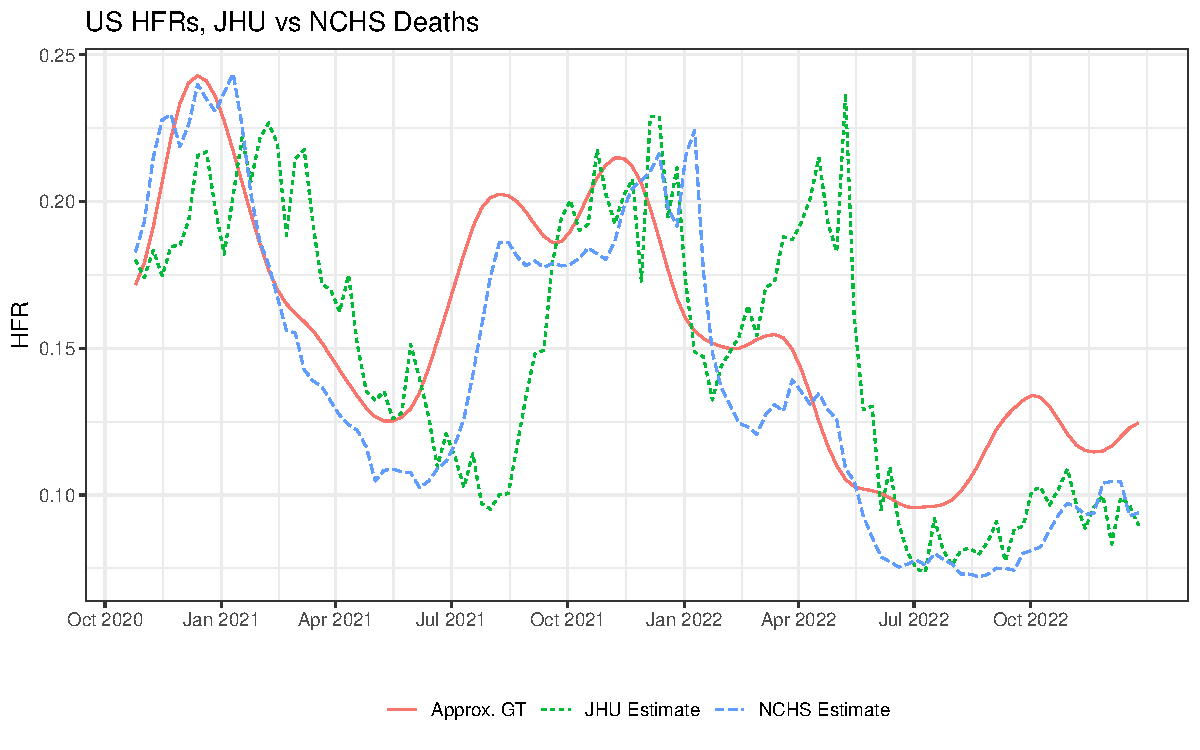
\includegraphics[width=0.7\linewidth]{Figs/Real/jhu_vs_nchs.pdf}
    \caption{Real-time Lagged Ratios, JHU vs NCHS deaths. Seven-day smoothing with 19- and 11-day lags, respectively.}
    \label{fig:jhu_vs_nchs}
\end{figure}


\subsection{Alternative ground truth}\label{apx:alt_gt}

\begin{figure}
    \centering
    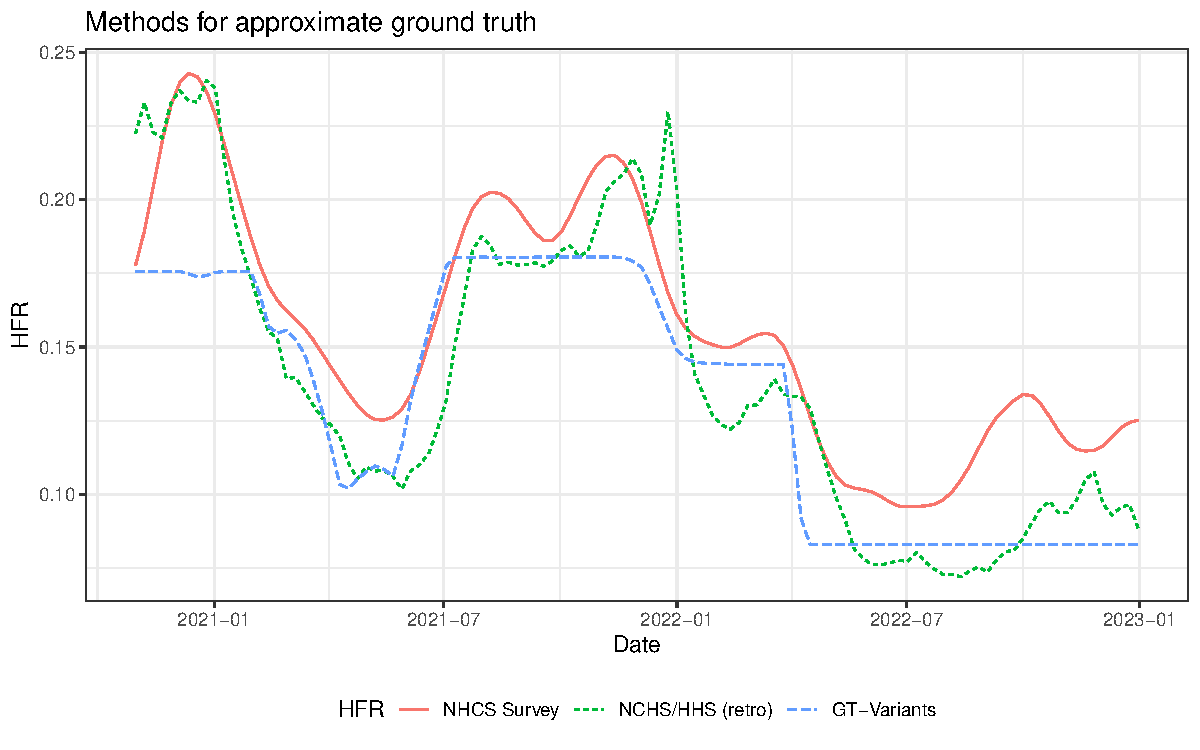
\includegraphics[width=0.8\linewidth]{Figs/Real/ApproxGT.pdf}
    \caption{Methods for Retrospective Ground Truth HFRs.}
    \label{fig:approxGT}
\end{figure}

We considered two retrospective approaches to approximate the ground truth national HFRs over time. The first approach took lagged ratios with aggregate deaths from NCHS. NCHS is a better resource than JHU because it uses death counts from the date they actually occurred, not merely reported. In addition, we take a forward-looking ratio, which is retrospective insofar as it uses data after time $t$ to estimate the HFR.
% Unlike the real-time estimates, we  method is forward-looking and . 

\begin{equation}\label{eq:LaggedRetro}
    \hat{p}_t^{\text{LaggedRetro}} = \frac{Y_{t+L}}{X_t}
\end{equation}
% \noindent Equation \eqref{eq:LaggedRetro} is retrospective because it uses data after time $t$, and therefore is not applicable in real-time. 

The second approach computed a single HFR for each major variant, then mixing by the proportions of variants in circulation. Formally, let $\hat{p}_j$ approximate the HFR of variant $j$; let $v_t^j$ be its proportion of cases at time $t$, where $\sum_j v_t^j = 1 \; \forall t$. The HFR estimate is

$$\hat{p}_t^{\text{Var}} = \sum_j v_t^j \hat{p}_j.$$

Each variant's HFR $\hat p_j$ was defined as the ratio of total NCHS deaths and HHS hospitalizations during the period where it accounted for over 50\% of activate cases. The case proportions $v_t^j$ were obtained from \texttt{covariants.org}. To ensure estimates were reasonable, we only considered the 4 largest variants: The original strain, Alpha, Delta, and Omicron. Because Omicron began with an enormous surge that quickly subsided, we split it into early and late periods at April 1, 2022, following \citep{adjei2022mortality}.

Figure \ref{fig:approxGT} displays the three curves approximating the true HFRs. They have nontrivial differences in magnitude, but move more or less in conjunction. To validate our results, we primarily used the rescaled NHCS HFRs as the least problematic of the three. The retrospective NCHS ratios are subject to statistical bias, expressed in \eqref{eq:LagBias}. The variant-based HFRs are flatter, as they do not account for other sources of variability. Therefore, they do not explain for the statistical bias within each variant period, which arises due to changes in the underlying severity rate.  %unreasonably flat

\section{Robustness checks}\label{apx:robustness}
\subsection{Data source}
The results in Section~\ref{sec:results_real} use hospitalization and death counts available in real time. To investigate the sensitivity of our findings, we recomputed the lagged and convolutional ratios, this time using the finalized aggregates. Figure \ref{fig:rt_and_final} shows the estimates with real-time and finalized counts track very closely to one another. Therefore, the observed bias in \ref{fig:basic_est_vs_gt_figs} cannot be attributed to reporting quirks.

The one period where the curves are significantly different from one another is in March 2022. While the HFRs from finalized counts steadily rise, the real-time estimates sharply fall then immediately bounce back. This sudden drop is due to a brief period in which reported death counts were suddenly too low (Fig. \ref{fig:source}. This is corrected in the finalized counts, hence their smooth HFRs. Removing this artifact further reinforces the bias trends described in Section~\ref{sec:ws_analysis}.

\begin{figure}
     \centering
     \begin{subfigure}[b]{0.45\linewidth}
         \centering
         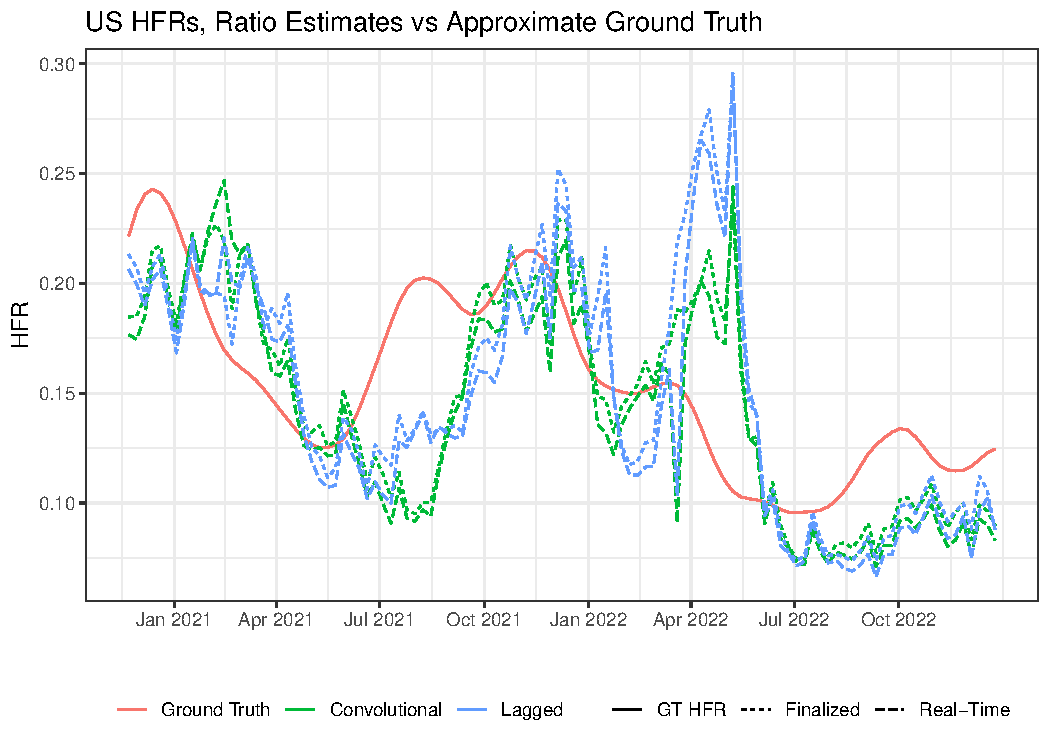
\includegraphics[height=6cm]{Figs/Real/US_ests_realtime_both.pdf}
         \caption{HFR estimates with real-time and finalized counts.}
         \label{fig:rt_and_final}
     \end{subfigure}
     \hfill
     \begin{subfigure}[b]{0.45\linewidth}
         \centering
         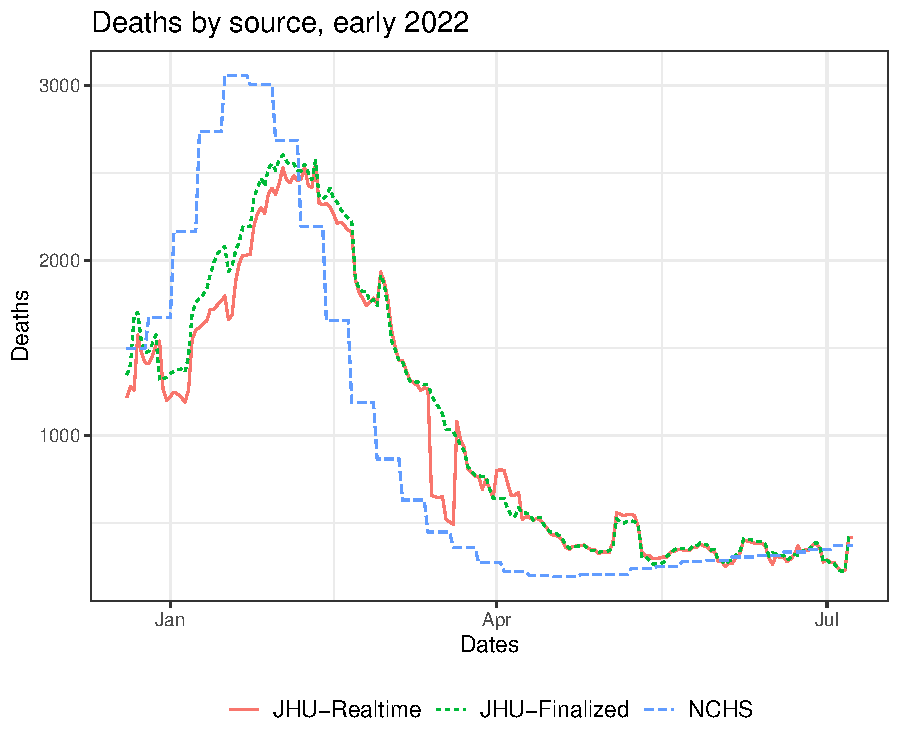
\includegraphics[height=6cm]{Figs/Real/death_curves.pdf}
         \caption{Aggregate deaths by data source and report time.}
         \label{fig:source}
     \end{subfigure}
        \caption{Convolutional ratio estimates are biased regardless of which delay distribution is selected.}
        \label{fig:real_time_vs_finalized}
\end{figure}


\subsection{Hyperparameters}
In this section we demonstrate the robustness of our findings against choices of hyperparameters. (All results are with the finalized version of JHU deaths.) First, Figure \ref{fig:window} plots performance over choices of window size parameter. We analyze smoothed versions of the lagged estimator

\begin{equation}\label{eq:laggedSmooth}
    \hat{p}_t^{\ell, W} = \frac{\sum_{s=t-w+1}^{t} Y_s}{\sum_{s=t-w+1}^{t} X_{s-\ell}},
\end{equation}
\noindent as well as the convolutional estimator
\begin{equation}\label{eq:convSmooth}
    \hat{p}_t^{\gamma, W} = \frac{\sum_{s=t-w+1}^{t} Y_s}{\sum_{s=t-w+1}^{t} \sum_{k=0}^d X_{s-\ell-k}\gamma_k}.
\end{equation}

\noindent Results are very similar, indicating the bias does not disappear when smoothing over a longer history. 

\begin{figure}
    \centering
    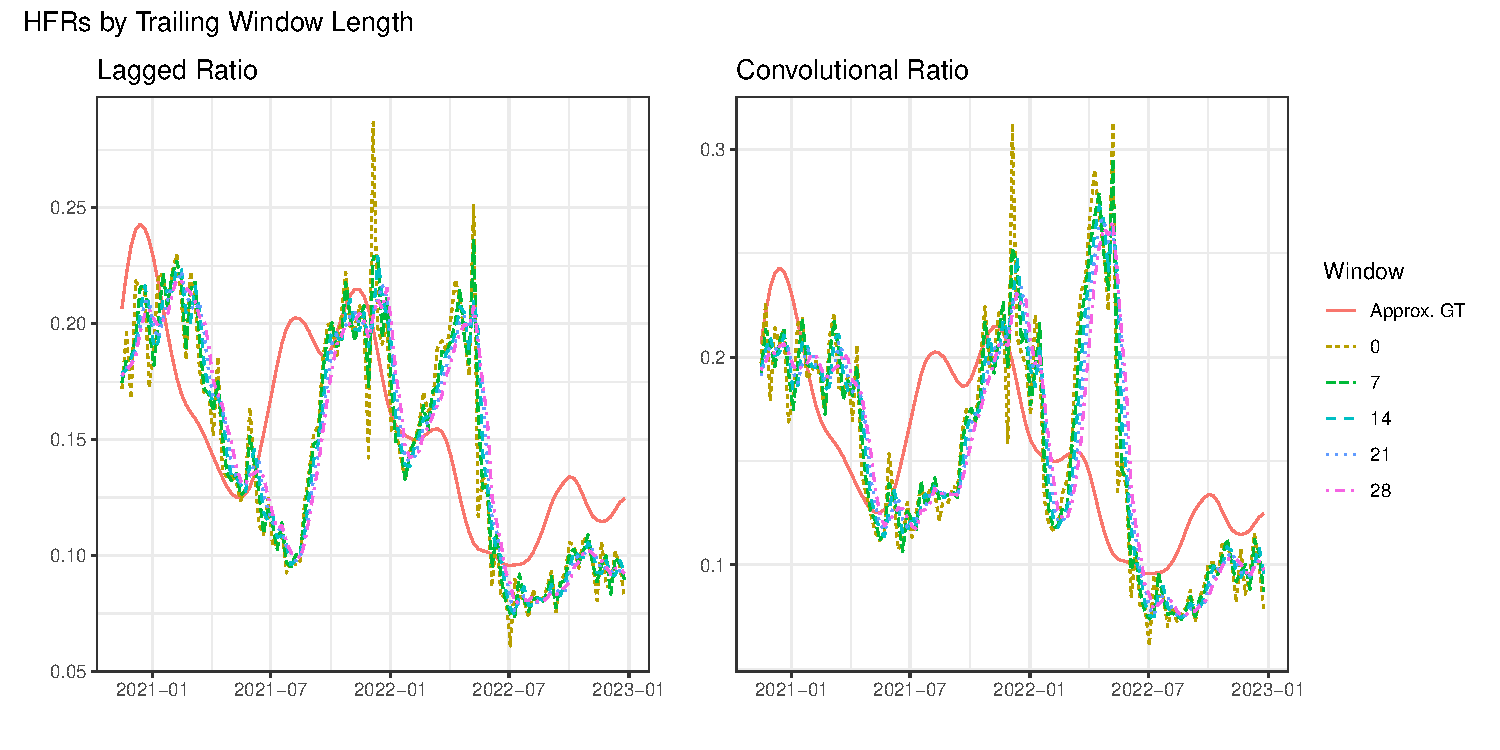
\includegraphics[width=0.75\linewidth]{Figs/Real/window_size.pdf}
    \caption{The length of the trailing window bears little impact on the findings.}
    \label{fig:window}
\end{figure}

We next examine the time-to-death hyperparameters: The lag $\ell$ for the lagged ratio and delay distribution $\pi$ for the convolutional ratio. Figure \ref{fig:lag} displays HFR estimates with lags ranging from 2 to 5 weeks. Unlike the window size, changing this parameter leads to different behavior across lags. Some choices are better than others; a 28-day lag, for example, falls appropriately in winter 2021 and rises less slowly during Delta. However, all are biased to varying degrees, most notably the huge spurious surge in spring 2022.

\begin{figure}
    \centering
    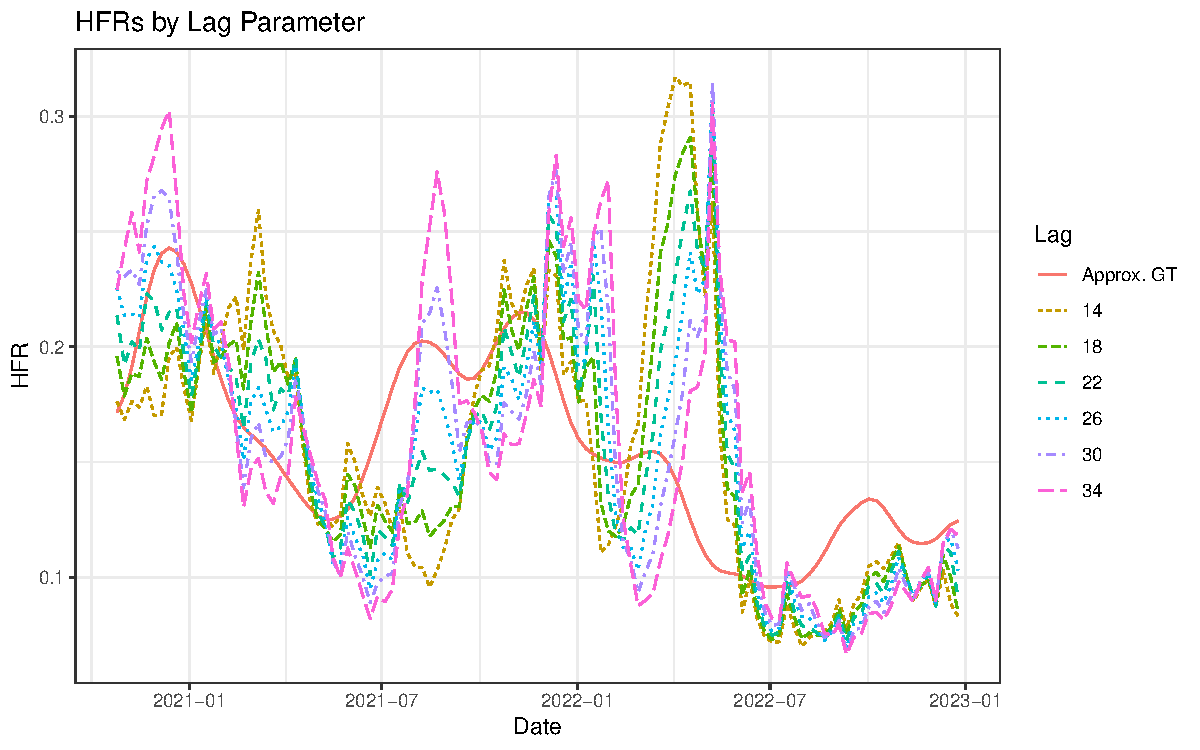
\includegraphics[width=0.7\linewidth]{Figs/Real/hfrs_by_lag.pdf}
    \caption{HFRs are biased regardless of what lag parameter is selected.}
    \label{fig:lag}
\end{figure}


Figure \ref{fig:delays} compares the performance of the convolutional ratio across different choices of delay distribution. We kept the discrete gamma shape for each, but varied the mean and standard deviation. As before, Figure \ref{fig:delay1} kept the standard deviation to 90\% of the mean, per \citet{UKdelay}. We also evaluated with a more compact delay distribution in \ref{fig:delay2}. 

% \begin{figure}
%     \centering
%     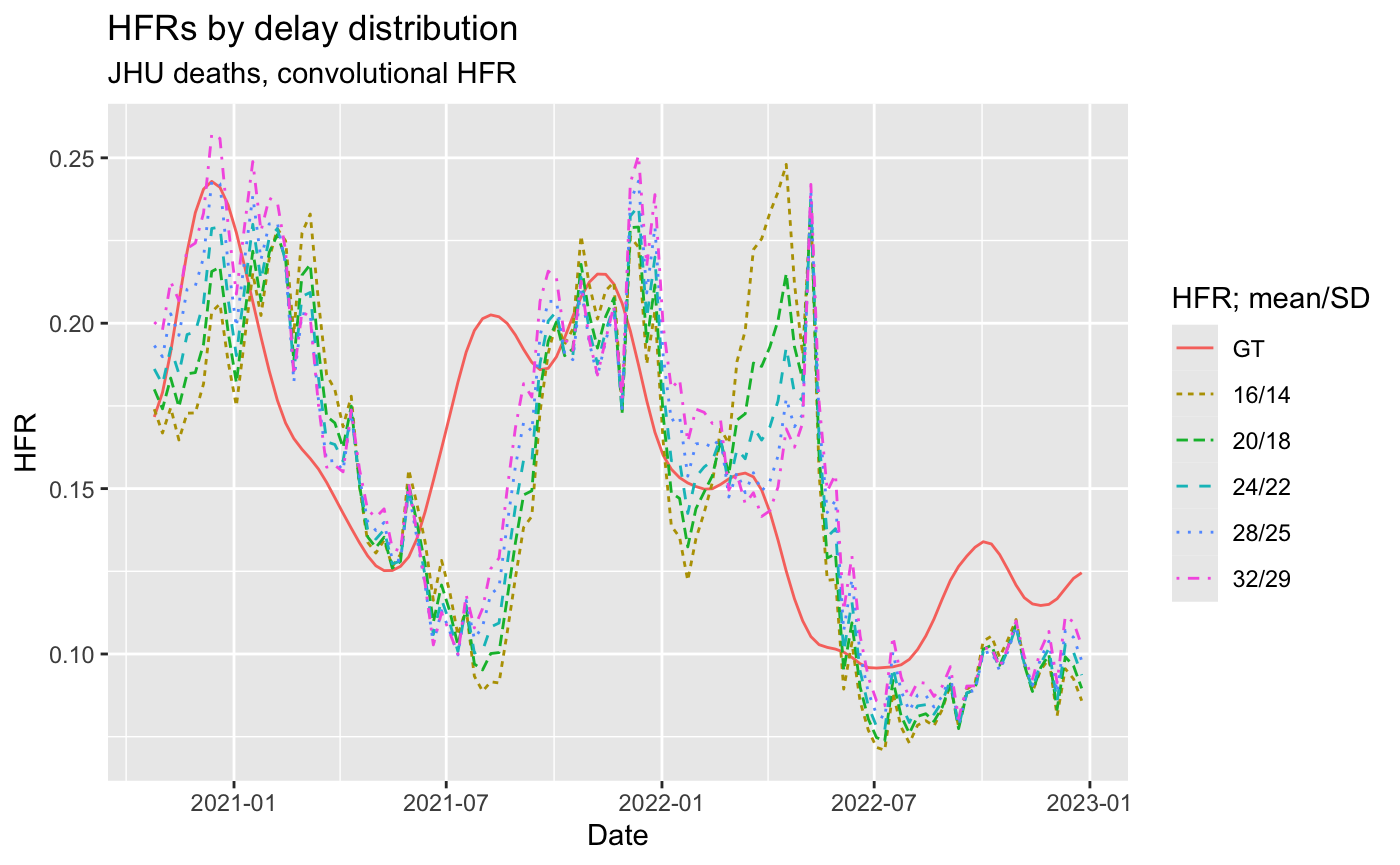
\includegraphics[width=0.7\linewidth]{Figs/Real/hfrs_by_delay.pdf}
%     \caption{HFRs are biased regardless of what delay distribution is selected.}
%     \label{fig:delay}
% \end{figure}

\begin{figure}
     \centering
     \begin{subfigure}[b]{0.45\linewidth}
         \centering
         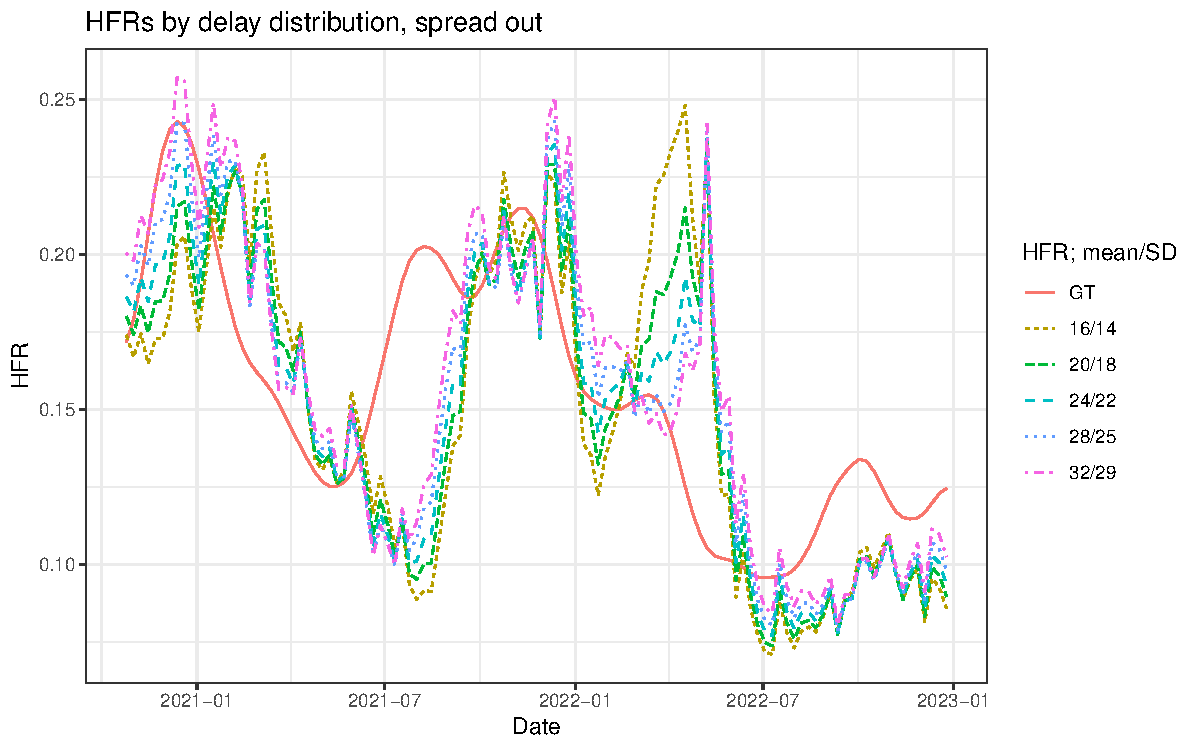
\includegraphics[width=\linewidth]{Figs/Real/hfrs_by_delay1.pdf}
         \caption{SD is $0.9\times$mean.}
         \label{fig:delay1}
     \end{subfigure}
     \hfill
     \begin{subfigure}[b]{0.45\linewidth}
         \centering
         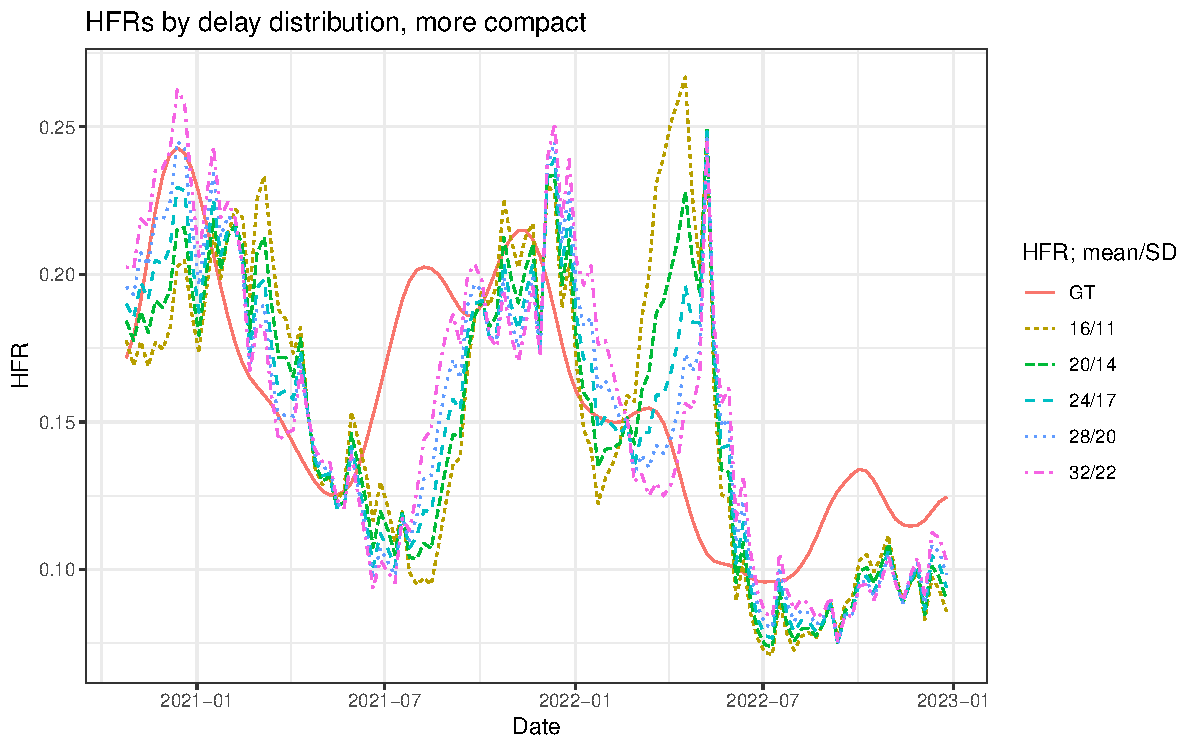
\includegraphics[width=\linewidth]{Figs/Real/hfrs_by_delay2.pdf}
         \caption{SD is $0.7\times$mean.}
         \label{fig:delay2}
     \end{subfigure}
        \caption{Convolutional ratio estimates are biased regardless of which delay distribution is selected.}
        \label{fig:delays}
\end{figure}
All HFR estimates in the figures are significantly biased. Regardless of delay distribution, the ratios are negatively biased during the onset of Delta, and surge after the peak of Omicron. This indicates the bulk of the error is fundamental to the estimator, and cannot be attributed to model misspecification. 

Comparing to the approximate ground truth HFRs from NHCS, performance improved slightly with a longer delay distribution than the purported mean of 20 days. Its mean absolute error was 0.031, whereas the delay distribution with mean 28 and standard deviation 25 had a MAE of 0.27. Nevertheless, this difference is relatively small, with the alternative delay distribution still showing similar bias.

\subsection{Geography}

Next, we repeat our analysis on different geographies, finding similar trends. We repeated our computations on the 6 largest US states with the same lag and delay distribution, with finalized death counts from JHU. Because the NHCS survey was conducted on a subset of hospitals meant to represent the US at large, it may poorly approximate the HFRs for individual states. A better state-level source is the retrospective lagged ratio (\ref{eq:LaggedRetro}) using NCHS deaths. Figure \ref{fig:state-level} compares this rough ground truth with the real-time estimates. For both NCHS and JHU deaths, we again take the lag that maximizes cross-correlation with hospitalizations; the standard deviation of the delay distribution is 0.9 times the mean. 

 \begin{figure}
     \centering
     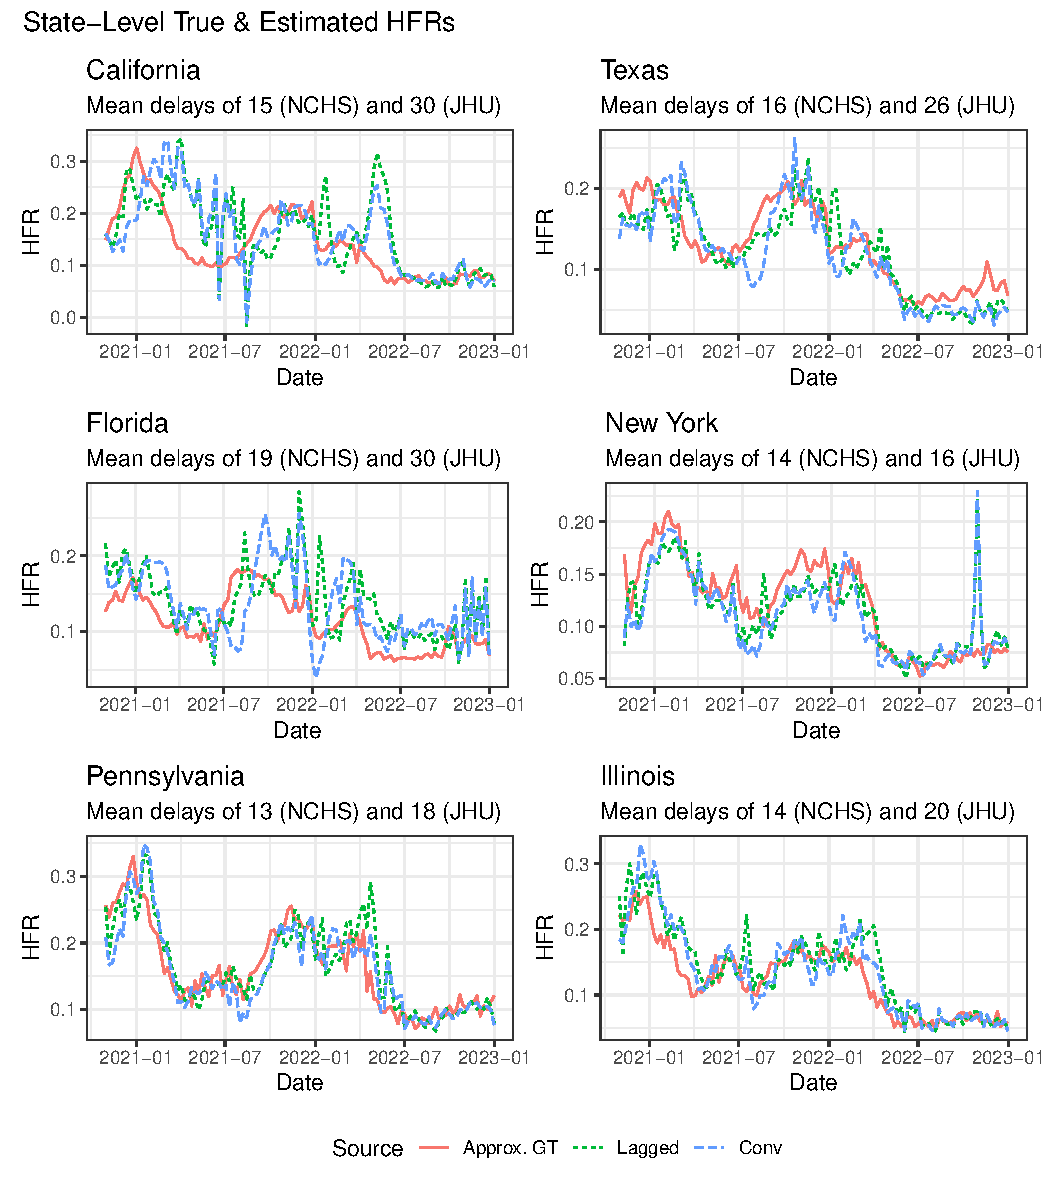
\includegraphics[width=0.8\linewidth]{Figs/Real/state_level_hfrs.pdf}
     \caption{HFRs by individual states. Comparing retrospective estimates with NCHS against real-time estimates with JHU.}
     \label{fig:state-level}
 \end{figure}

Several states have similar biases as the US results (Fig. \ref{fig:basic_est_vs_gt}). Ratios in California, Texas, and Florida all are slow to detect the uptick in HFR during Delta; they also spike during Omicron in California, and to a lesser extent Florida. Note these states are the ones with the largest optimal lags, an estimate of the average time to death. As our simulated examples have shown, the shape of the delay distribution is a key factor behind the degree of bias. In contrast, New York, Pensylvania, and Illinois have mean delays of at most 17. While their HFRs are still biased, they are relatively close to the NCHS curve. This suggests that fatality ratios are generally less trustworthy in states that take longer to report deaths.

\section{Miscellaneous results}\label{apx:misc}
\subsection{Alternative lag on simulation}
\begin{figure}
    \centering
    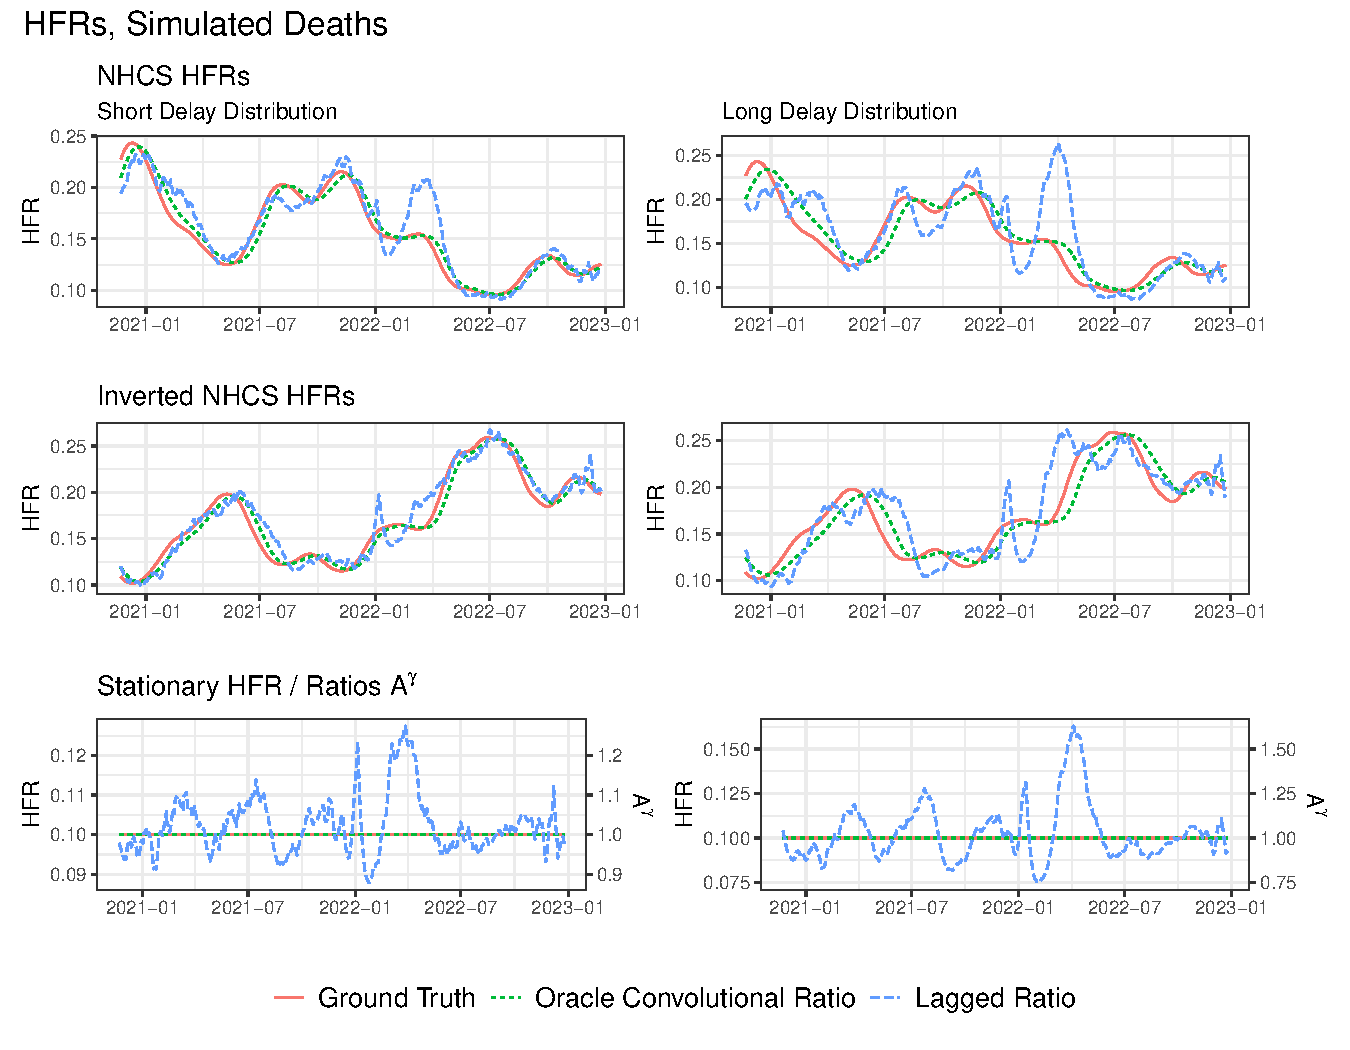
\includegraphics[width=\linewidth]{Figs/Simulated/simulated_results_corr_lag.pdf}
    \caption{Lag chosen as mean of delay distribution. Same simulated data as Section~\ref{sec:results_sim}.}
    \label{fig:sims_mean_lag}
\end{figure}

Figure \ref{fig:sims_mean_lag} presents the simulation results from Section~\ref{sec:results_sim} when the lag is the mean of the delay distribution. It clearly indicates the lagged ratio is not markedly better under this lag. This is in step with Figure \ref{fig:lag}, which demonstrated that its performance on real data are robust to choice of lag.

\subsection{Further analysis}\label{apx:analysis}
In this section, we present examples that further explain the well-specified bias. These are more contrived that the ones in Section~\ref{sec:ws_analysis}, for example using unrealistic delay distributions. Nevertheless, their bias can be simplified to simple analytic formulas, isolating the three contributing factors.
% In contrast to the examples in~\ref{sec:ws_analysis}, the ones here use contrived delay distributions and

\begin{figure}
     \centering
     \begin{subfigure}[b]{0.45\linewidth}
         \centering
         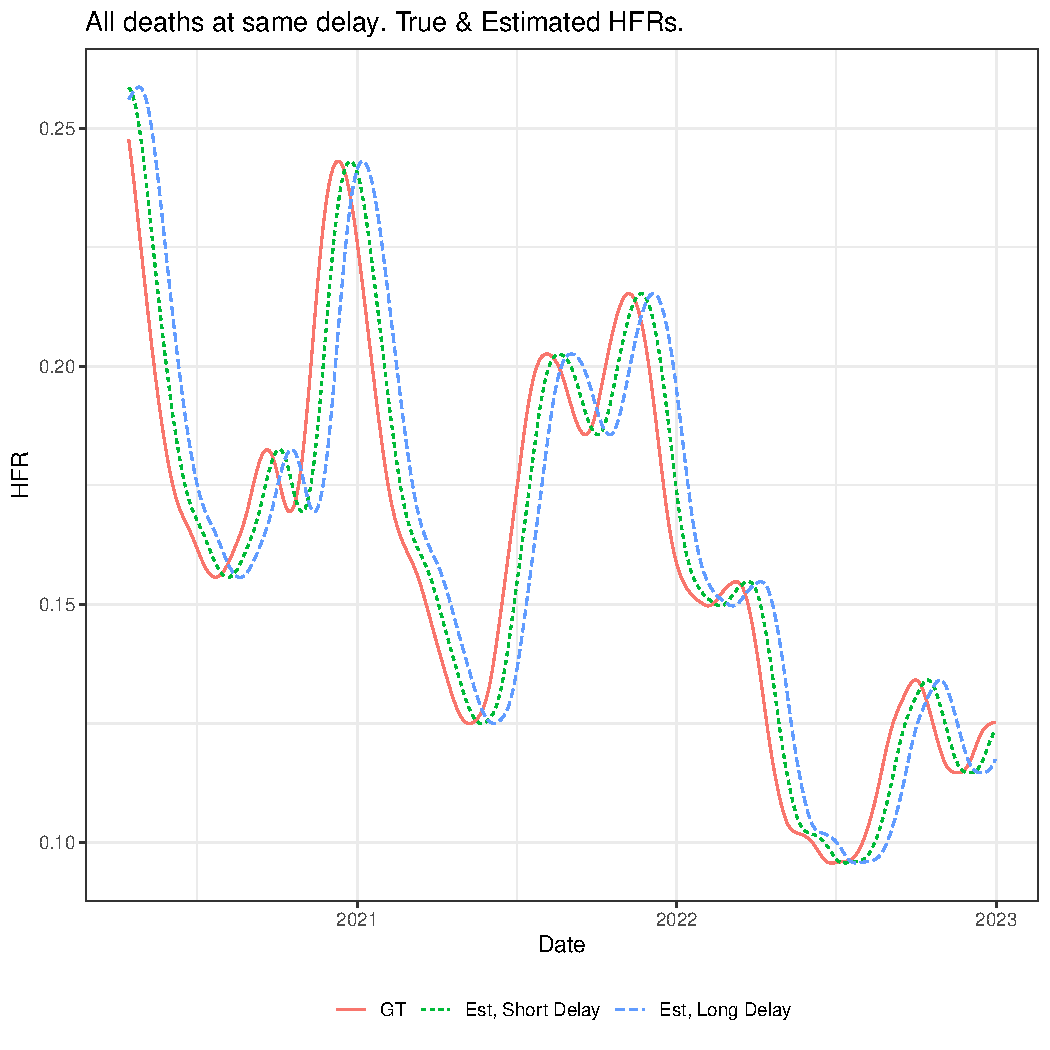
\includegraphics[width=\linewidth]{Figs/Simulated/sim_onehot.pdf}
         \caption{All deaths after $\ell$ days. HFR ratios equivalent; plotting delays of $\ell=14$ and 28 days.}
         \label{fig:onehot}
     \end{subfigure}
     \hfill
     \begin{subfigure}[b]{0.45\linewidth}
         \centering
         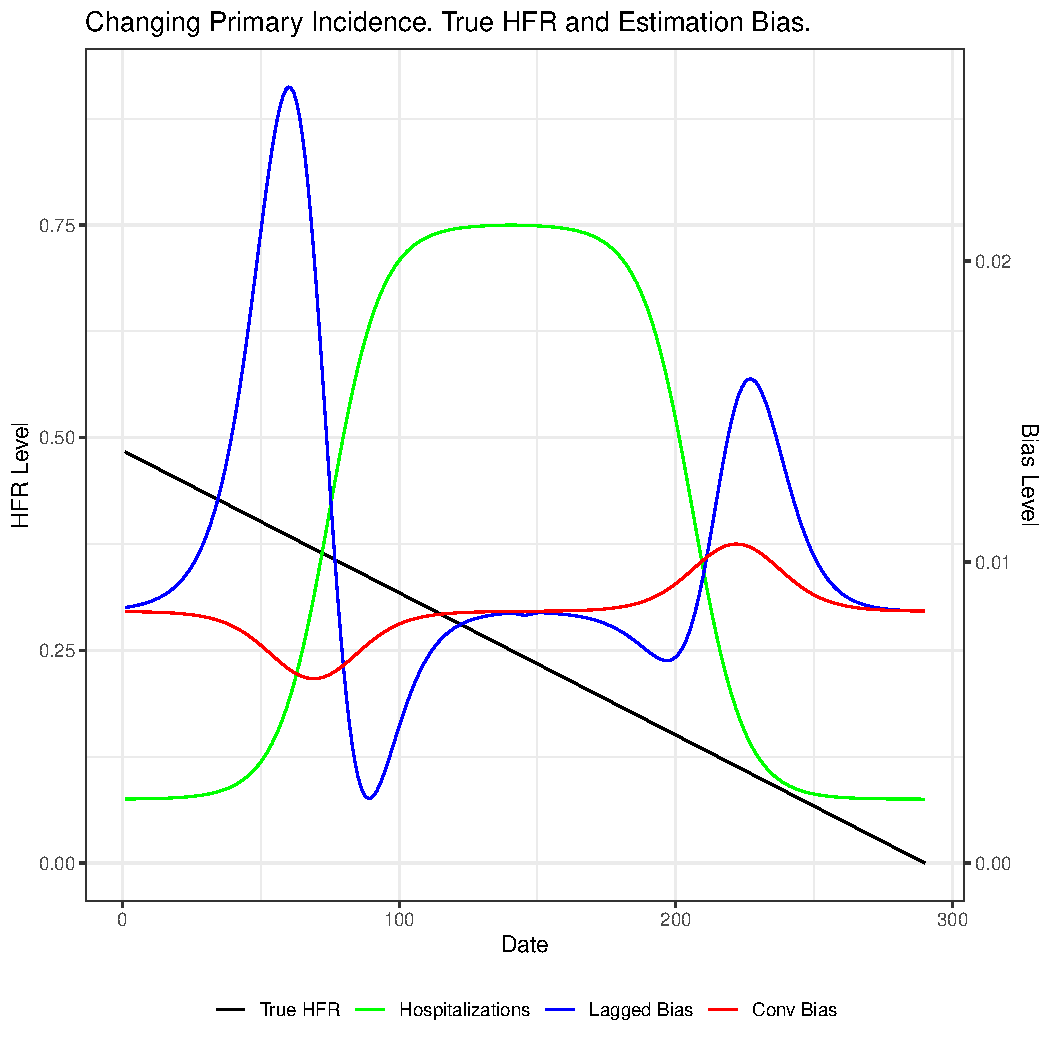
\includegraphics[width=\linewidth]{Figs/Simulated/sim_chging_primary.pdf}
         \caption{Changing primary incidence. Plotting bias of lagged and convolutional ratios.}
         \label{fig:chging_primary}
     \end{subfigure}
        \caption{Toy examples of biased severity rates.}
        \label{fig:bias_ex}
\end{figure}


To elucidate the relationship between changing severity rates and the ratio estimators' bias, consider the trivial case where all secondary events occur after exactly $\ell$ days with no noise. By definition, $\pi_k = \mathds{1}\{k=\ell\}$, so the convolutional and lagged ratios are both $\hat{p}_t = \frac{X_{t-\ell}p_{t-\ell}}{X_{t-\ell}} = p_{t-\ell}$ presuming both have access to the oracle delay distribution. Figure \ref{fig:onehot} displays this with the approximate ground truth HFRs from NHCS. 

In this case, the bias is the change in the true severity rate $p_{t-\ell} - p_t$. The estimator is unbiased only when the severity rate is stationary. Otherwise, for example, the ratio will be 20\% too low if the true severity rate was 20\% lower $\ell$ days ago. 

Intuitively, severity rates may be less similar to the present value $p_t$ further back in time. In this simple example, the bias $p_{t-\ell}-p_t$ is generally larger when $\ell=28$ than $\ell=14$ (Fig \ref{fig:onehot}). This expresses the observation that estimates with heavier-tailed delay distributions tend to have more bias. 

Section~\ref{sec:ws_analysis} claims that changes in primary incidence levels affect the magnitude of bias for the convolutional ratio. Here, we present simple examples that formalize this claim. First assume primary incidence is constant, in which case the convolutional and lagged ratios are equal. The time series factors neatly out of the bias expression  Proposition \ref{thm:OracleBias}:
$$\text{Bias}(\hat{p}_t^{\gamma}) = \text{Bias}(\hat{p}_t^\ell) = \Big(\sum_{k=0}^d \pi_k p_{t-k}\Big)-p_t.$$
\noindent This is the difference between a weighted average of previous severity rates and the present. Weights for the historical rates are given by the delay distribution, providing further justification for its central role in the bias. 

Next, suppose half of the secondary events occur immediately after the primary event ($t=0$), and the other half after $d$ days. Further assume $p_{t-d}\neq p_t$, so there is some degree of bias. Then
\begin{align*}
    \lvert\text{Bias}(\hat{p}_t^{\gamma})\rvert &= \frac{\frac{1}{2}\big\lvert X_{t}(p_t-p_t) + X_{t-d}(p_{t-d}-p_t)\big\rvert}{\frac{1}{2}(X_{t}+X_{t-d})} \\
    &=\frac{X_{t-d}\lvert p_{t-d}-p_t\rvert}{X_{t-d}(1+\frac{X_{t}}{X_{t-d}})} = \frac{\lvert p_{t-d}-p_t \rvert}{1+\frac{X_{t}}{X_{t-d}}}
\end{align*}

The absolute bias is monotonically decreasing in $\frac{X_{t}}{X_{t-d}}$, the proportion change in primary incidence. Rising primary incidence ($\frac{X_{t}}{X_{t-d}}>1)$ yields less bias, while falling levels yield more.

Figure \ref{fig:chging_primary} displays this setting. Hospitalizations are defined as $X = \sigma(s)*9000+1000$, where $\sigma$ is the sigmoid function and $s$ takes 300 evenly spaced steps from -9 to 7. The true HFRs fall from 0.5 to 0 over the same number of even steps. Indeed, the convolutional ratio's bias dips as hospitalizations rise, and rises as they fall. 

The figure also plots with lagged ratio with $\ell=\frac{d}{2}$, the mean of the delay distribution. When daily hospitalizations are close to constant, the two estimators converge towards the same ratio. During periods of change, however, the lagged estimator has different bias. It first moves upwards --- the opposite direction as the convolutional bias --- with far greater magnitude. This can be explained by the ratio $A_t^\ell = \frac{X_{t-2\ell}+X_t}{2X_{t-\ell}}$ from Proposition \ref{thm:MispBias}. As hospitalizations begin to steeply rise, $X_{t-2\ell}$ and $X_{t-\ell}$ are similar, but $X_t > X_{t-\ell}$. Hence, $A_t^\ell>1$, contributing positive bias to both the oracle and misspecification terms. As hospitalizations level out near the top, $A_t^\ell < 1$, hence the bias falling lower. The opposite pattern occurs as hospitalizations fall. 

% Since the convolutional ratio uses the true delay distribution, it has oracle bias in Proposition \ref{thm:MispBias}. The lagged ratio has lag at the mean of the delay distribution, $\ell=\frac{d}{2}$. Its behavior can be explained by the ratio $A_t^\ell = \frac{X_{t-2\ell}+X_t}{2X_{t-\ell}}$. As hospitalizations begin to steeply rise, $X_{t-2\ell}$ and $X_{t-\ell}$ are similar, but $X_t > X_{t-\ell}$. Therefore $A_t^\ell>1$, inflating the positive oracle bias term and adding misspecification bias. As hospitalizations level out near the top, $A_t^\ell < 1$, hence the bias falling lower. The opposite pattern occurs as hospitalizations fall. 


\end{document}
